\documentclass[aspectratio=169,11pt]{beamer}

\usetheme{Boadilla}
\usecolortheme{default}
\usefonttheme{professionalfonts}
\setbeamertemplate{navigation symbols}{}

\usepackage[utf8]{inputenc}
\usepackage[english]{babel}
\usepackage{amsmath,amssymb}
\usepackage{booktabs}
\usepackage{graphicx}
\usepackage{tikz}
\usetikzlibrary{positioning}
\usepackage[notocbib]{apacite}
\usepackage{hyperref}
\IfFileExists{fontawesome5.sty}{\usepackage{fontawesome5}}{}

\graphicspath{{plots/}{../plots/}}

\definecolor{itamblue}{RGB}{13,33,161}
\definecolor{itamlight}{RGB}{234,239,255}
\definecolor{itamaccent}{RGB}{6,62,134}

\setbeamercolor{structure}{fg=itamblue}
\setbeamercolor{title}{fg=white,bg=itamblue}
\setbeamercolor{frametitle}{fg=white,bg=itamblue}
\setbeamercolor{palette primary}{fg=white,bg=itamblue}
\setbeamercolor{palette secondary}{fg=white,bg=itamaccent}
\setbeamercolor{palette tertiary}{fg=white,bg=itamblue}
\setbeamercolor{palette quaternary}{fg=white,bg=itamaccent}
\setbeamercolor{block title}{fg=white,bg=itamblue}
\setbeamercolor{block body}{fg=black,bg=itamlight}

\setbeamertemplate{itemize item}{\color{itamblue}$\blacktriangleright$}
\setbeamertemplate{itemize subitem}{\color{itamblue}$\bullet$}

\newcommand{\itamlogopath}{logo-ITAM.png}
\IfFileExists{logo-ITAM.png}{}{\renewcommand{\itamlogopath}{../logo-ITAM.png}}

\newcommand{\thesisbib}{biblo}
\IfFileExists{biblo.bib}{}{\renewcommand{\thesisbib}{../biblo}}
\newcommand{\githubicon}{\textbf{GitHub}}
\IfFileExists{fontawesome5.sty}{\renewcommand{\githubicon}{\faGithub}}{}

\addtobeamertemplate{background canvas}{}{%
\begin{tikzpicture}[remember picture,overlay]
\node[anchor=north east,xshift=-0.12cm,yshift=-0.10cm] at (current page.north east)
{\includegraphics[height=0.72cm]{\itamlogopath}};
\end{tikzpicture}
}

\title[Thesis]{Modelado de rendimientos financieros:\\volatilidad condicional, colas pesadas y dependencia multivariada}
\author[F. P\'erez Mill\'an]{Fernando P\'erez Mill\'an\\[0.5em]\small Asesor: Dr.~Carlos Vladimir Rodr\'iguez Caballero}
\institute[]{Instituto Tecnol\'ogico Aut\'onomo de M\'exico}
\date{}

\begin{document}

\begin{frame}[plain]
\titlepage
\end{frame}

\begin{frame}{Agenda}
\tableofcontents[sections={1-7}]
\end{frame}

\section{Objective and Data}
\begin{frame}{Objective}
\begin{itemize}\setlength{\itemsep}{1em}
\item Provide a coherent, step-by-step \textbf{recipe} for financial return modeling at the undergraduate level.
\item Follow one consistent path: empirical characterization, univariate modeling, forecast evaluation, and multivariate extension.
\item Keep a dual lens throughout:
\begin{itemize}
\item \textbf{Statistical validity} of model assumptions.
\item \textbf{Risk-management usefulness} (VaR/ES forecasts).
\end{itemize}
\end{itemize}
\end{frame}

\begin{frame}{Data}
\begin{block}{Data (Training set)}
\begin{itemize}
\item Daily returns: S\&P 500 and 10-year U.S. Treasury note index (SPBDU1BT).
\item Sample used across chapters: Jan 2014--Dec 2024.
\end{itemize}
\end{block}
\vspace{1.5em}
\begin{block}{Forecast (Test set)}
\begin{itemize}
\item Out-of-sample window: Jan 2025--Apr 2025 (81 observations).
\item Forecasts: 1-day-ahead density, VaR and ES (2.5\%).
\item Tests: Christoffersen tests, PIT diagnostics, KS, and DM comparison.
\end{itemize}
\end{block}
\end{frame}

\section{Empirical Characteristics of Returns}
\begin{frame}{Empirical Characteristics of Returns}
\begin{itemize}\setlength{\itemsep}{1em}
\item Stylized facts on S\&P 500 daily returns (2014--2024):
\begin{itemize}
\item Near-zero autocorrelation in raw returns.
\item Volatility clustering in squared returns.
\item Leverage effect.
\item Heavy tails, asymmetry, and high kurtosis.
\item Time-varying cross-asset dependence.
\end{itemize}
\item \textbf{These empirical characteristics serve as guidelines for what models should capture and replicate}
\end{itemize}
\end{frame}

\begin{frame}{Autocorrelation Patterns}
\begin{columns}[T]
\column{0.49\textwidth}
\centering
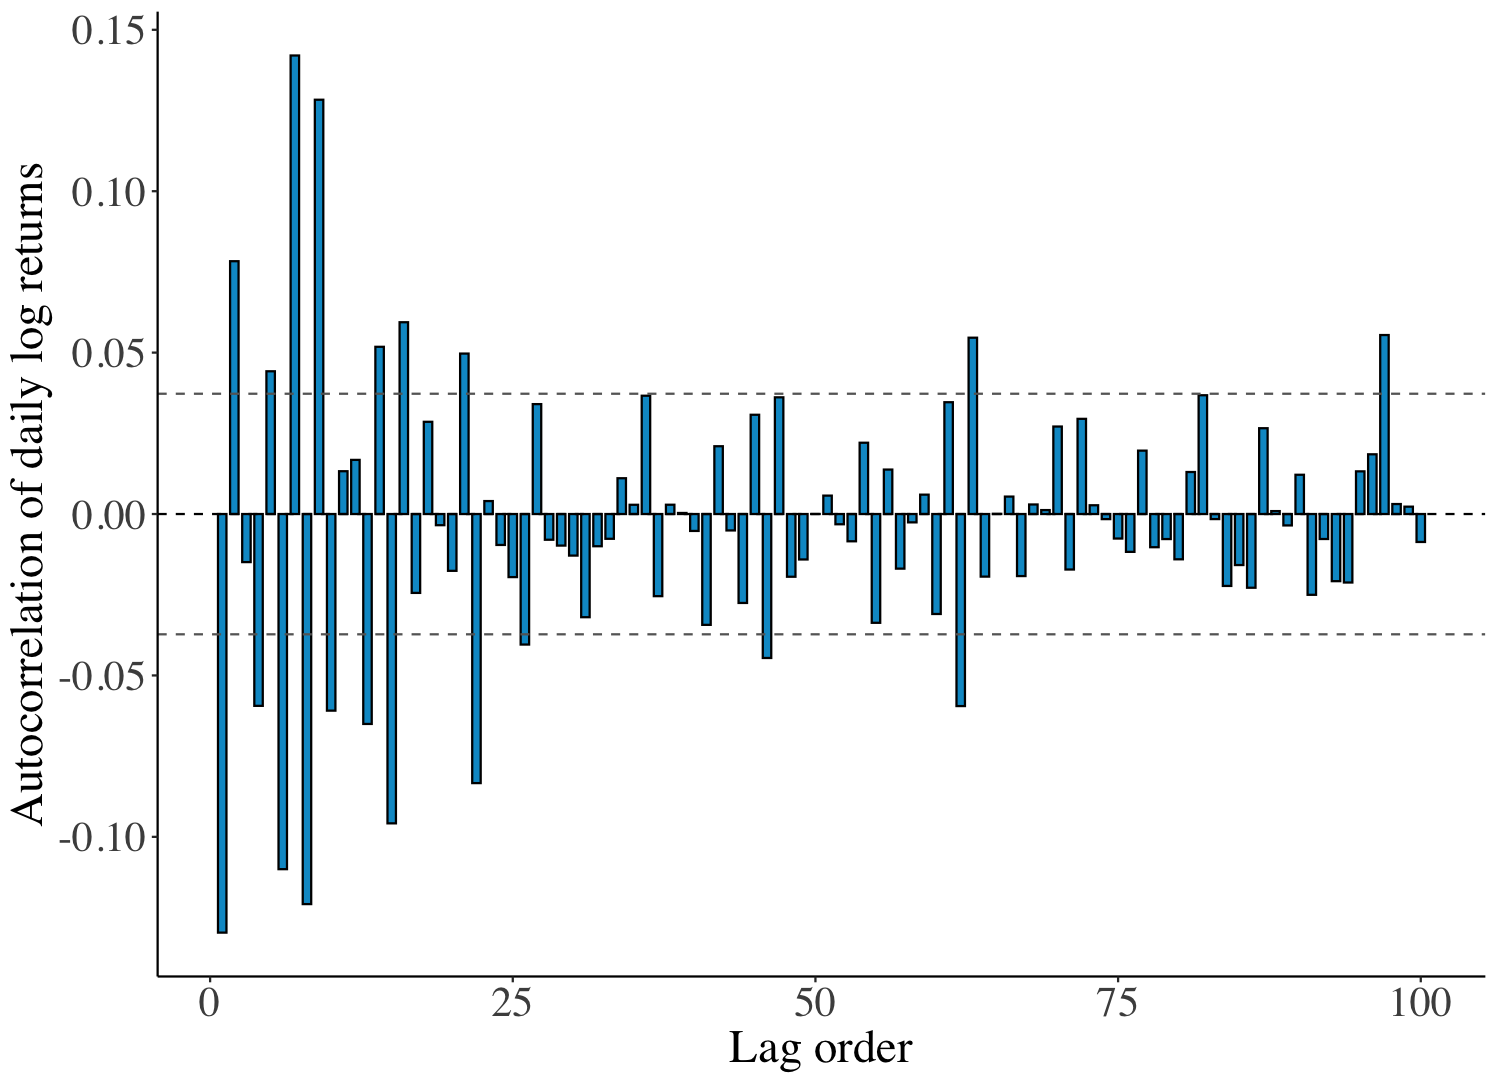
\includegraphics[width=0.95\linewidth]{1.1.png}
\vspace{0.1em}

\footnotesize Returns ACF
\column{0.49\textwidth}
\centering
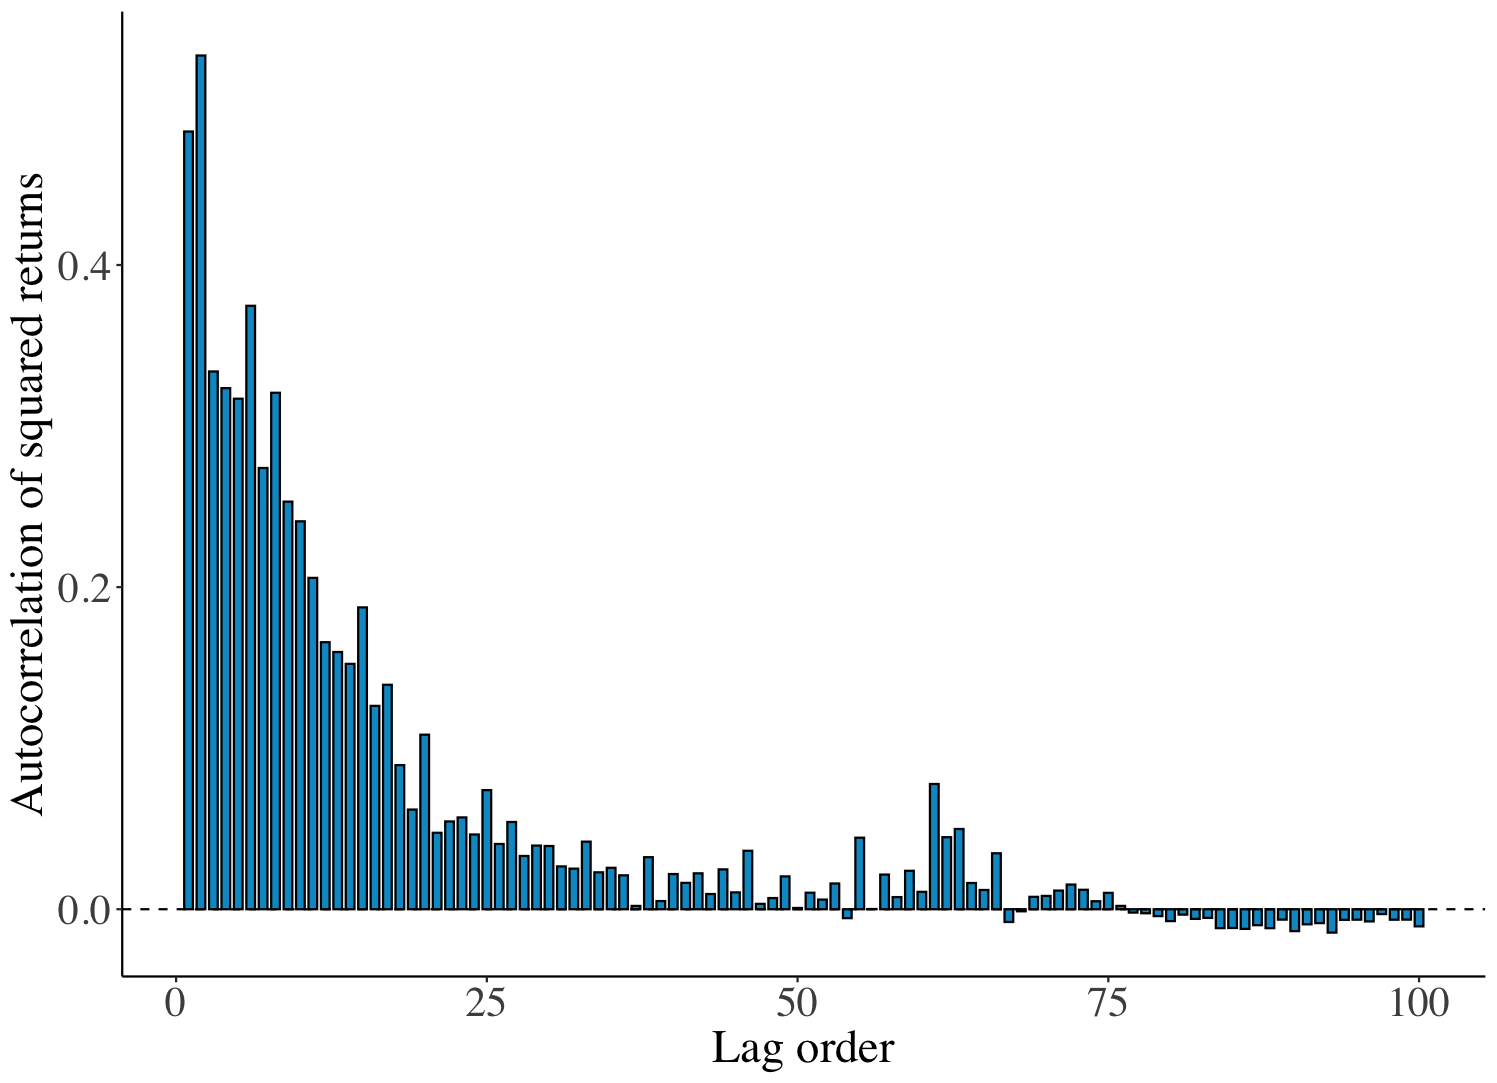
\includegraphics[width=0.95\linewidth]{1.3.png}
\vspace{0.1em}

\footnotesize Squared returns ACF
\end{columns}
\begin{itemize}
\item Returns: little linear predictability.
\item Squared returns: clear dependence and clustering.
\end{itemize}
\end{frame}

\begin{frame}{Distributional and Dependence Features}
\begin{columns}[T]
\column{0.49\textwidth}
\centering
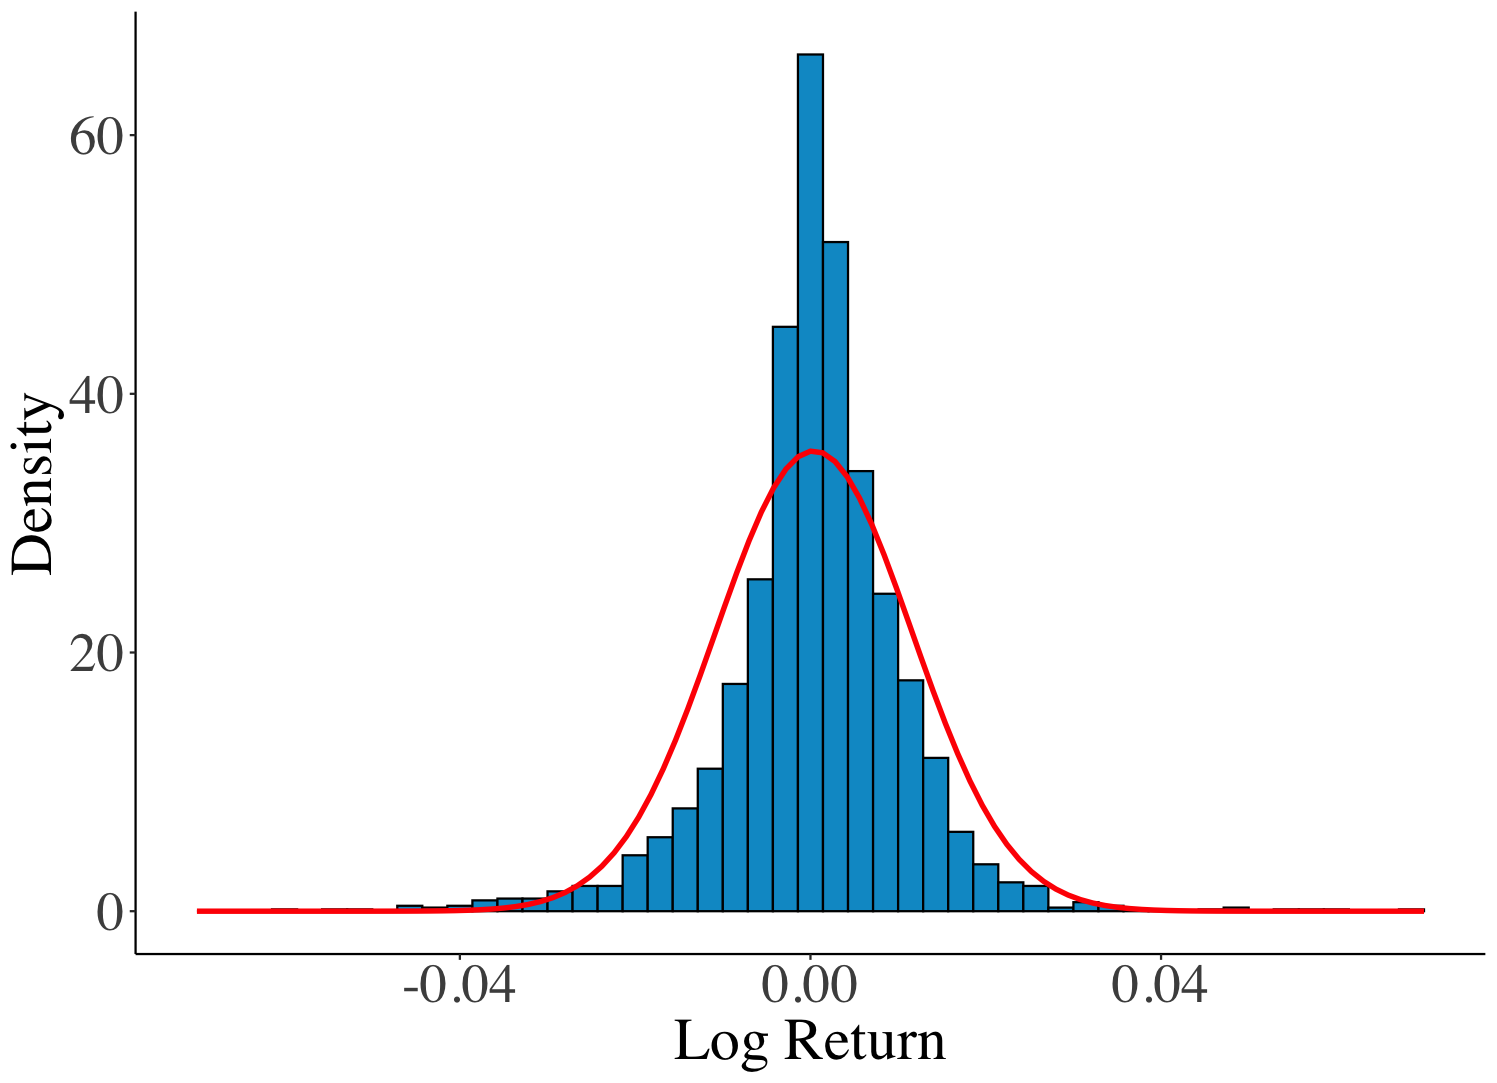
\includegraphics[width=0.94\linewidth]{1.2.png}
\column{0.49\textwidth}
\centering
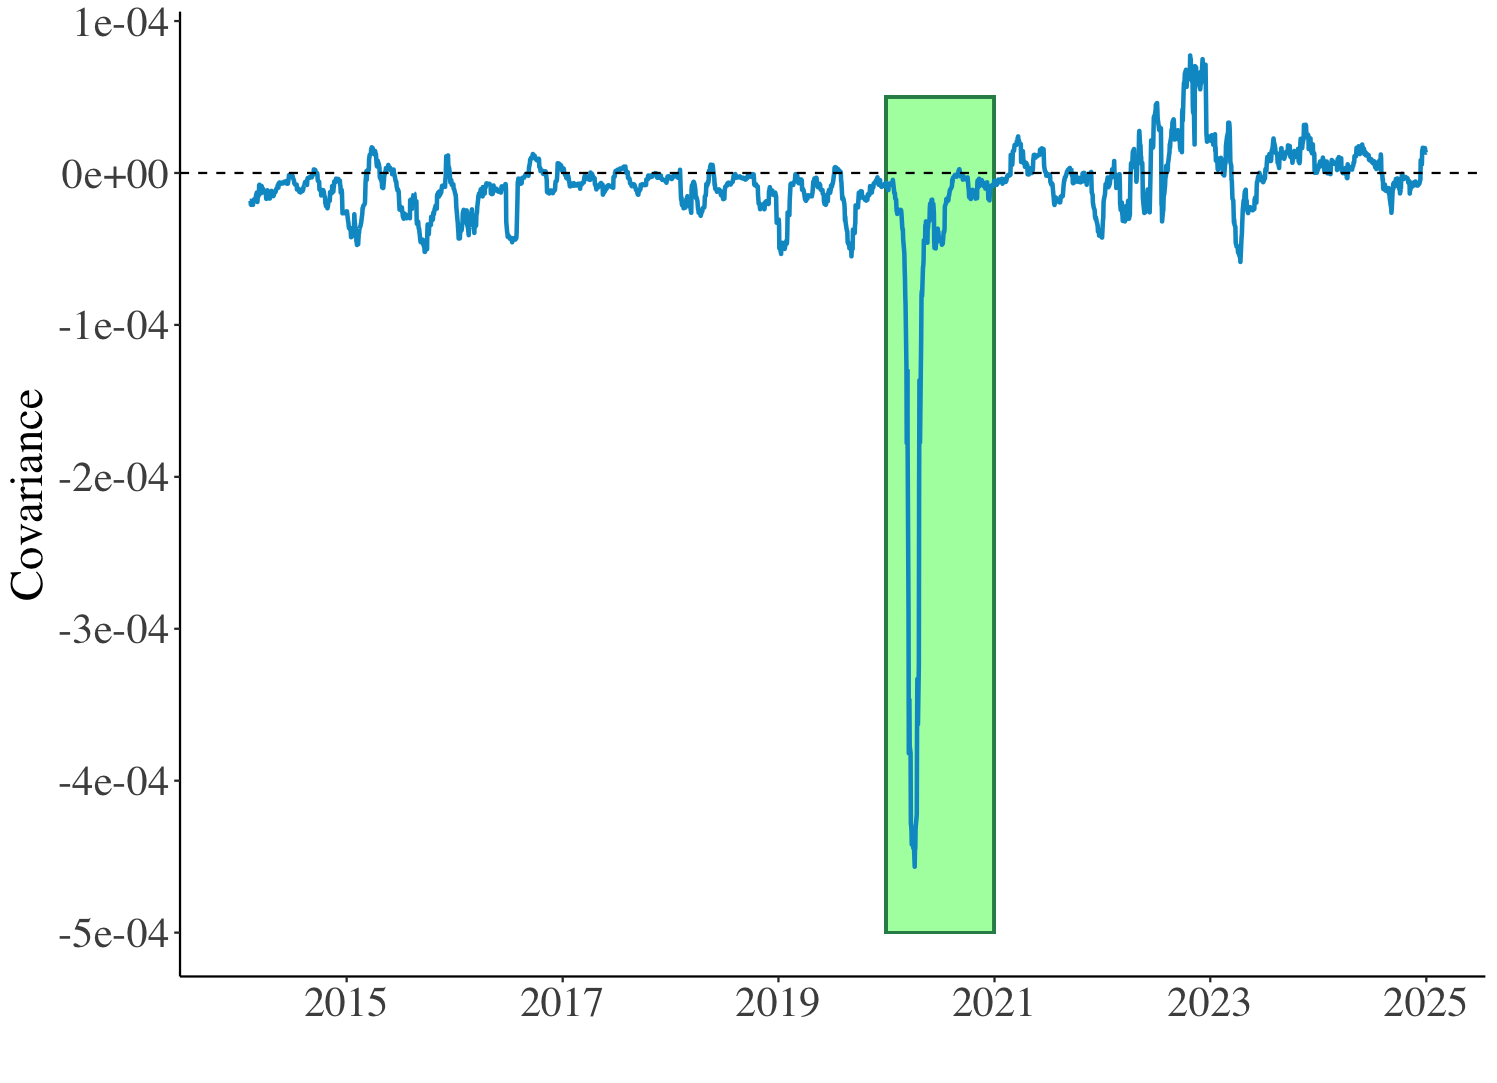
\includegraphics[width=0.94\linewidth]{1.4.png}
\end{columns}
\vspace{0.5em}
\begin{itemize}
\item The empirical distribution exhibits heavier tails than the normal distribution and asymmetry.
\item The correlation among assets appears to vary over time.
\end{itemize}
\end{frame}

\begin{frame}{Baseline Return Model}
\begin{block}{Return model}
\[
R_{t+1}=\sigma_{t+1}z_{t+1}, \qquad z_{t+1}\sim \text{i.i.d. }D(0,1)
\]
\end{block}
\end{frame}

\section{Volatility Modeling}
\begin{frame}{Volatility Modeling}
\begin{itemize}
\item Goal: model conditional variance \(\sigma_{t+1}^2\).
\item Ljung-Box on \(R_{t+1}^2\): strong evidence of conditional heteroskedasticity.
\item Two models:
\end{itemize}
\[
\textbf{GARCH(1,1):}\quad
\sigma^2_{t+1} = \omega + \alpha R_t^2 + \beta \sigma_t^2
\]
\[
\textbf{GJR-GARCH(1,1):}\quad
\sigma^2_{t+1} = \omega + \alpha R_t^2 + \alpha\theta I_tR_t^2 + \beta \sigma_t^2
\]
\begin{itemize}
\item Indicator variable: \(I_t=\mathbf{1}\{R_t<0\}\).
\begin{itemize}
\item If \(R_t<0\), \(I_t=1\) and shock impact is \(\alpha(1+\theta)R_t^2\).
\item If \(R_t\ge 0\), \(I_t=0\) and shock impact is \(\alpha R_t^2\).
\end{itemize}
\item GJR term (\(\theta>0\)) captures asymmetric (leverage) response.
\end{itemize}
\end{frame}

\begin{frame}{Parameter Estimation: QMLE}
\small
\begin{itemize}
\item Parameters: \(\vartheta=(\omega,\alpha,\beta)\) for GARCH(1,1), \(\vartheta=(\omega,\alpha,\beta,\theta)\) for GJR-GARCH(1,1).
\item \textbf{Quasi}-maximum likelihood: apply the normal MLE even if \(z_{t+1}\) is not normal (consistent estimates under correctly specified mean and variance).
\end{itemize}
Given a sample \(\{R_t\}_{t=1}^T\), the conditional log-likelihood under normality is
\[
\ell(\vartheta)
=-\frac{1}{2}\sum_{t=1}^T
\left[\log(2\pi)+\log(\sigma_t^2)+\frac{R_t^2}{\sigma_t^2}\right].
\]
The QMLE estimator solves
\[
\hat{\vartheta}=\arg\max_{\vartheta\in\Theta}\,\ell(\vartheta),
\]
subject to positivity and finite long-run variance restrictions.
\begin{itemize}
\item No closed-form maximizer: solved numerically, each \(\vartheta\) generating a full path \(\{\sigma_t^2\}_{t=1}^T\) via the volatility recursion.
\end{itemize}
\end{frame}

\begin{frame}{Estimated Dynamics (QMLE)}
\small
\begin{align*}
\text{GARCH(1,1):}\quad
\sigma^2_{t+1} &= 0.0000039 + 0.171R_t^2 + 0.794\sigma_t^2\\
\text{GJR-GARCH(1,1):}\quad
\sigma^2_{t+1} &= 0.0000040 + 0.054R_t^2 + 0.248I_tR_t^2 + 0.795\sigma_t^2
\end{align*}
\begin{columns}[T]
\column{0.49\textwidth}
\centering
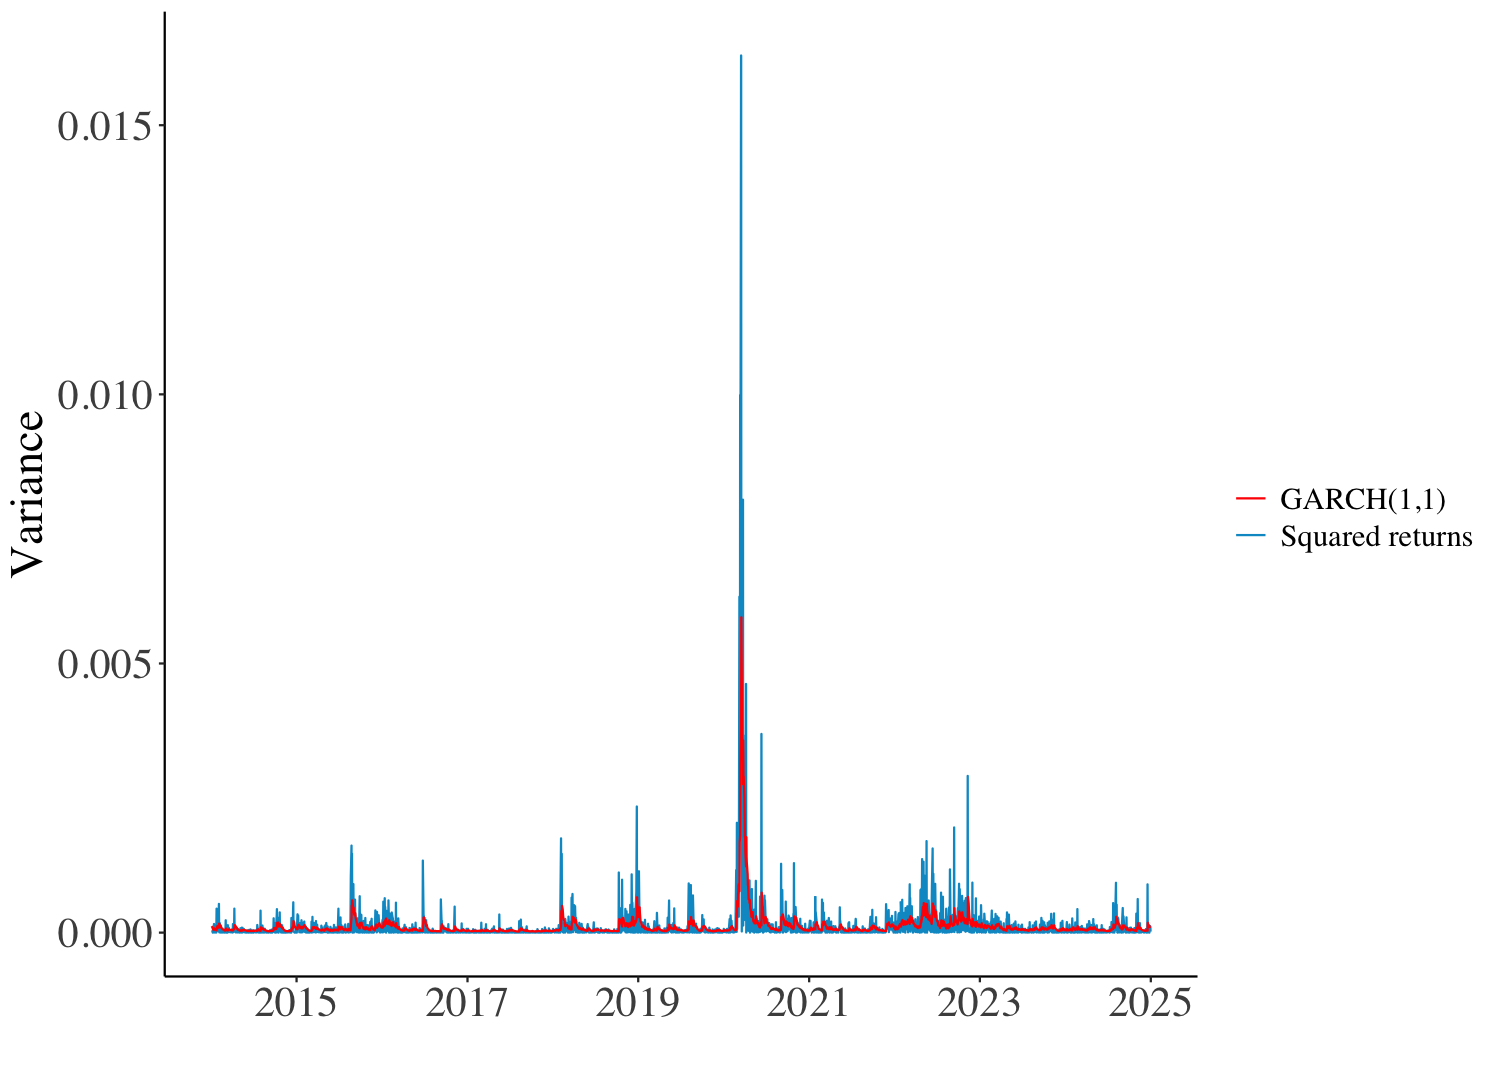
\includegraphics[width=0.92\linewidth]{2.2.png}
\column{0.49\textwidth}
\centering
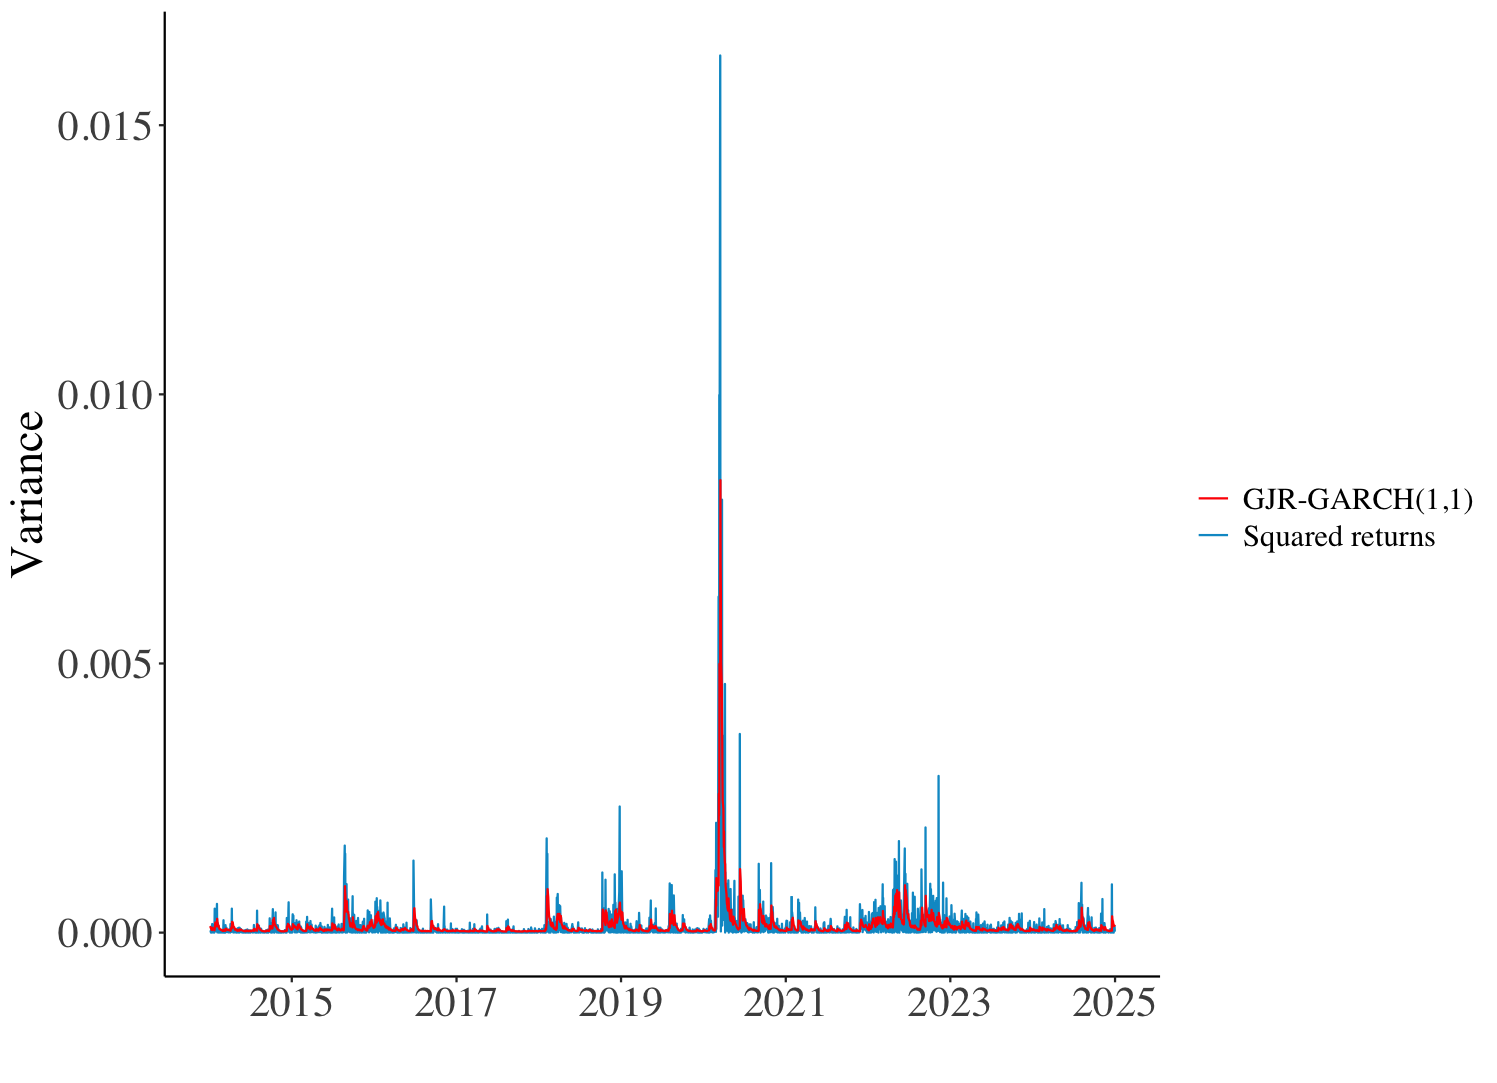
\includegraphics[width=0.92\linewidth]{2.3.png}
\end{columns}
\end{frame}

\begin{frame}{Key Takeaways on Volatility Modeling}
\begin{table}
\centering
\begin{tabular}{lc}
\toprule
Model & Mean QLIKE \\
\midrule
GARCH(1,1) & 1.6011 \\
GJR-GARCH(1,1) & 1.5673 \\
\bottomrule
\end{tabular}
\end{table}
\begin{itemize} \setlength{\itemsep}{1em}
\item LR test for extra GJR parameter: \(p<1\%\) (\citeA{Christoffersen2012} framework).
\item Both models absorb squared-return dependence.
\item Persistence is close to one, consistent with financial volatility behavior.
\end{itemize}
\end{frame}

\section{Shock Modeling}
\begin{frame}{Why Move Beyond Normal Shocks?}
\begin{columns}[T]
\column{0.49\textwidth}
\centering
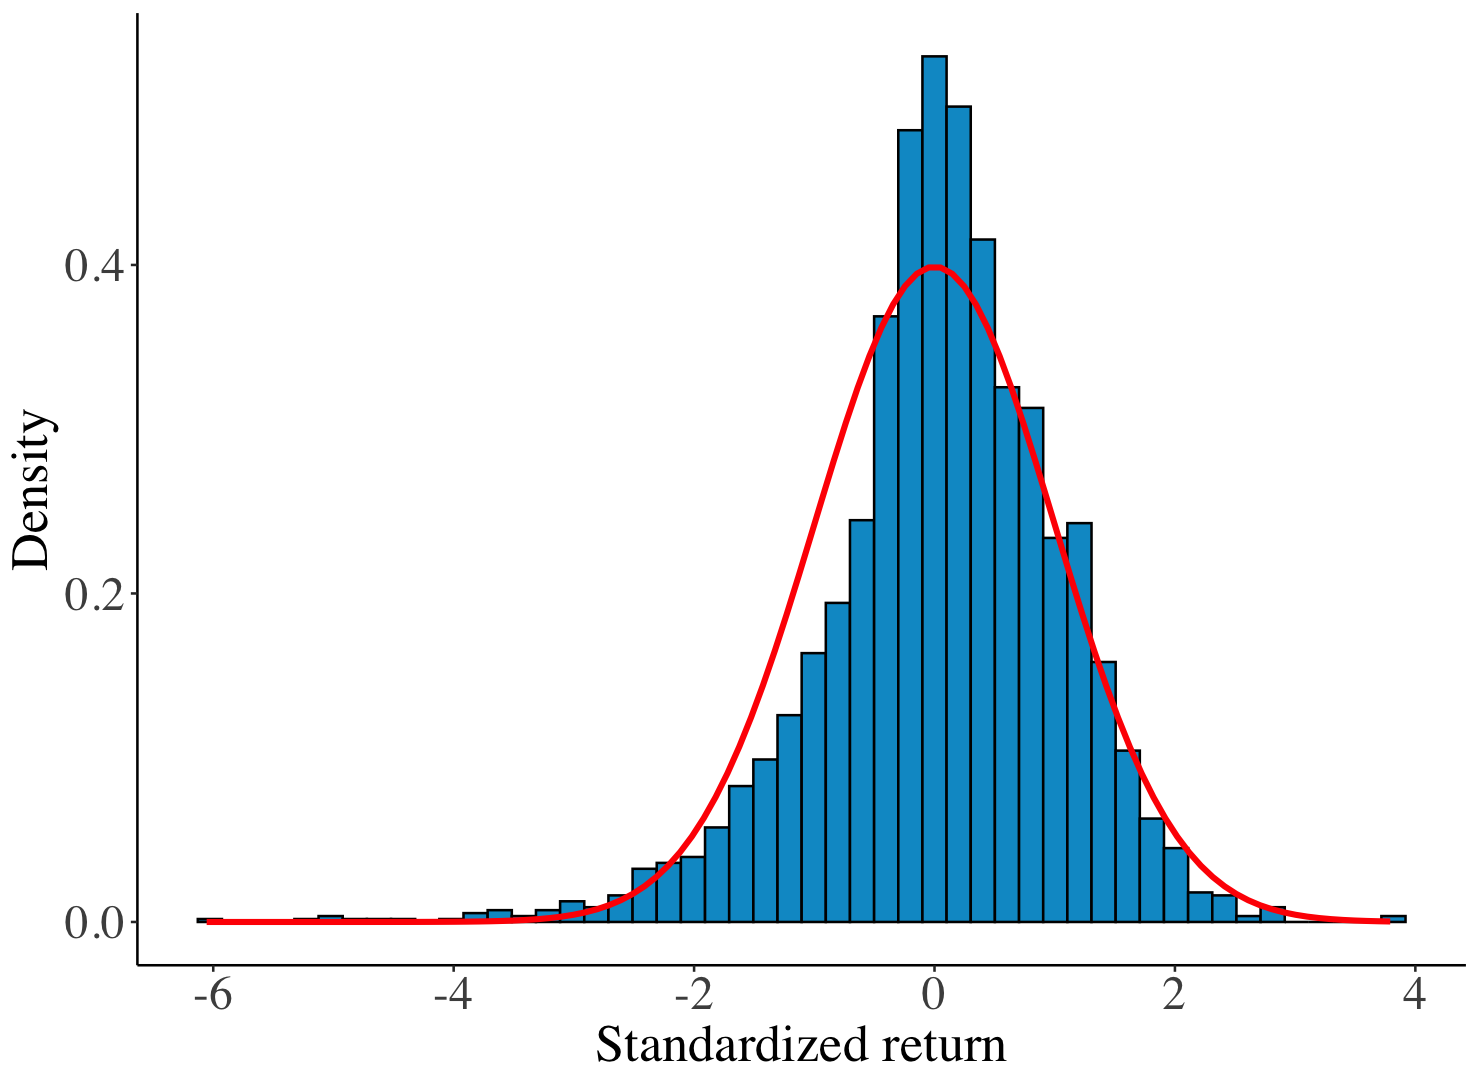
\includegraphics[width=\linewidth]{3.1.png}
\column{0.49\textwidth}
\centering
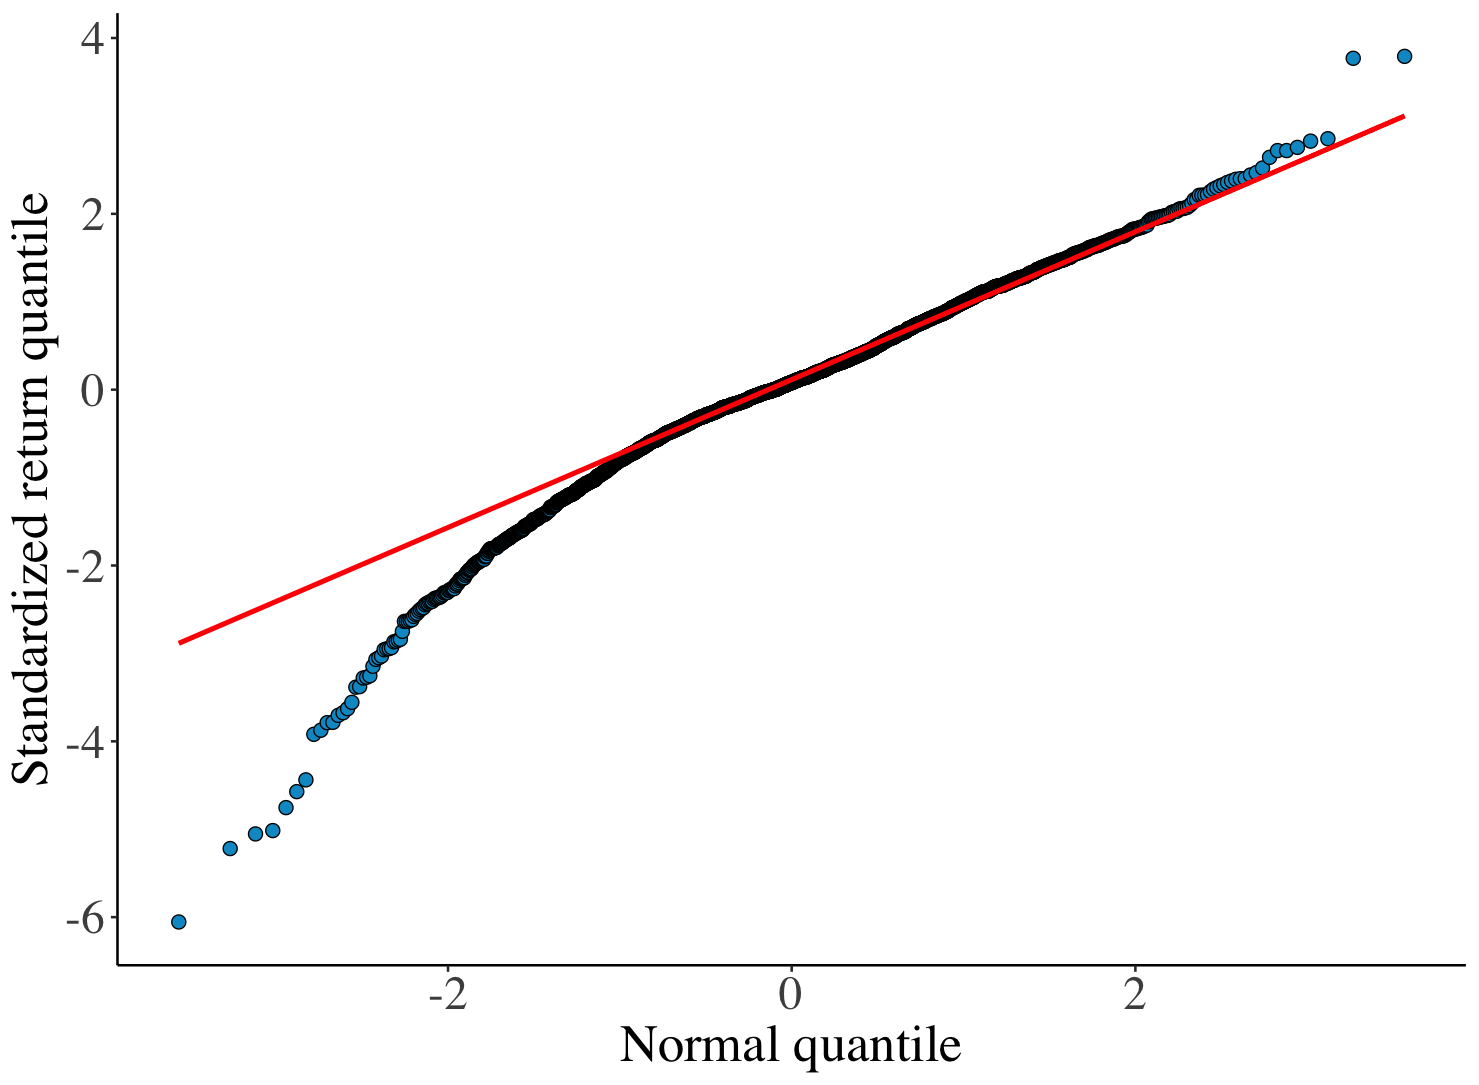
\includegraphics[width=\linewidth]{3.3.png}
\end{columns}
\begin{itemize}
\item Standardized residuals still show heavy tails and asymmetry.
\item Normality is strongly rejected (very small p-values in diagnostics).
\item Two alternatives considered: Asymmetric t and EVT-POT.
\end{itemize}
\end{frame}

\begin{frame}{Approach 1: Asymmetric t Shocks}
\small
\[
R_{t+1}=\sigma_{t+1}z_{t+1},\qquad z_{t+1}\sim \text{i.i.d. asyt}(d_1,d_2)
\]
\begin{itemize} \setlength{\itemsep}{1em}
\item Provides a skewed extension of the Student's t-distribution, enabling the modeling of both kurtosis and skewness observed in standardized returns.
\item Parameters estimated after volatility QMLE step.
\item Better center/tail fit than normal, but left tail remains underfit.
\end{itemize}
\end{frame}

\begin{frame}{Asymmetric t Fit Diagnostics}
\begin{columns}[T]
\column{0.49\textwidth}
\centering
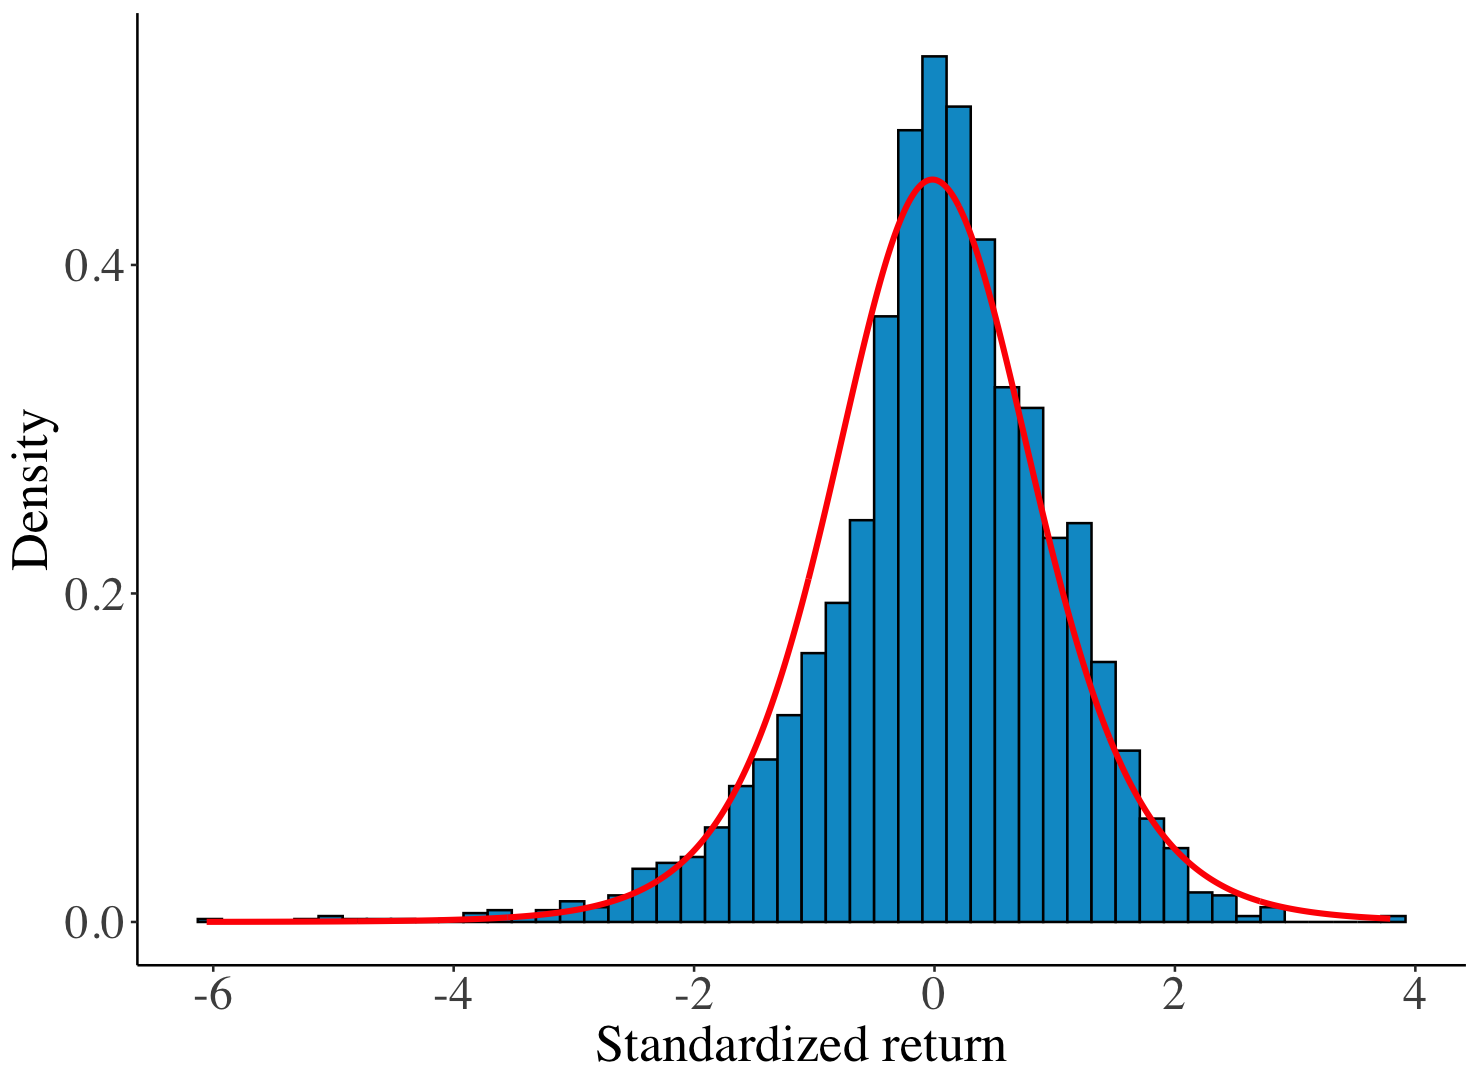
\includegraphics[width=0.95\linewidth]{3.5.png}
\column{0.49\textwidth}
\centering
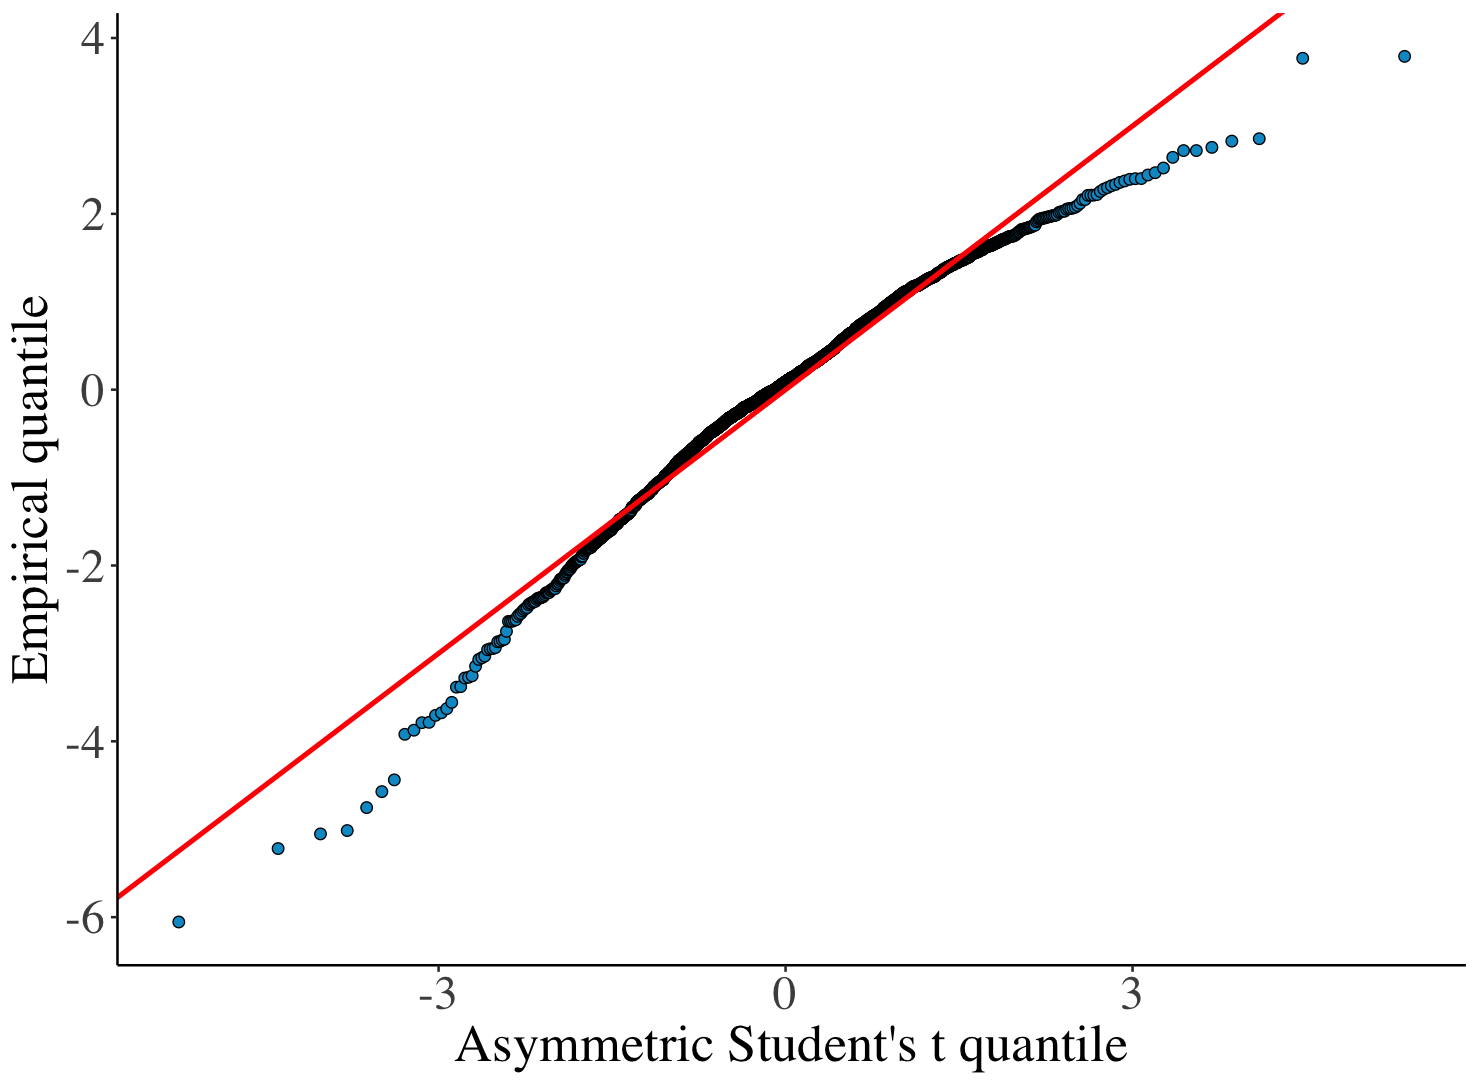
\includegraphics[width=0.95\linewidth]{3.7.png}
\end{columns}
\begin{itemize}
\item Good fit in the center and moderate tails.
\item Left extreme tail remains the main weakness for risk management.
\end{itemize}
\end{frame}

\begin{frame}{Approach 2: EVT (Peak-over-Threshold)}
\small
\[
-z_{t+1}\mid(-z_{t+1}>u)\sim \text{GPD}(\xi,\beta,u),\qquad u=1.8
\]
\[
f(y)=\frac{1}{\beta}\left(1+\frac{\xi(y-u)}{\beta}\right)^{-\left(1+\frac{1}{\xi}\right)},\quad y>u
\]
\begin{itemize} \setlength{\itemsep}{1em}
\item Focuses explicitly on left-tail risk, the critical region for VaR/ES.
\item Threshold chosen through mean excess function linearity.
\end{itemize}
\end{frame}

\begin{frame}{EVT Diagnostics}
\begin{columns}[T]
\column{0.49\textwidth}
\centering
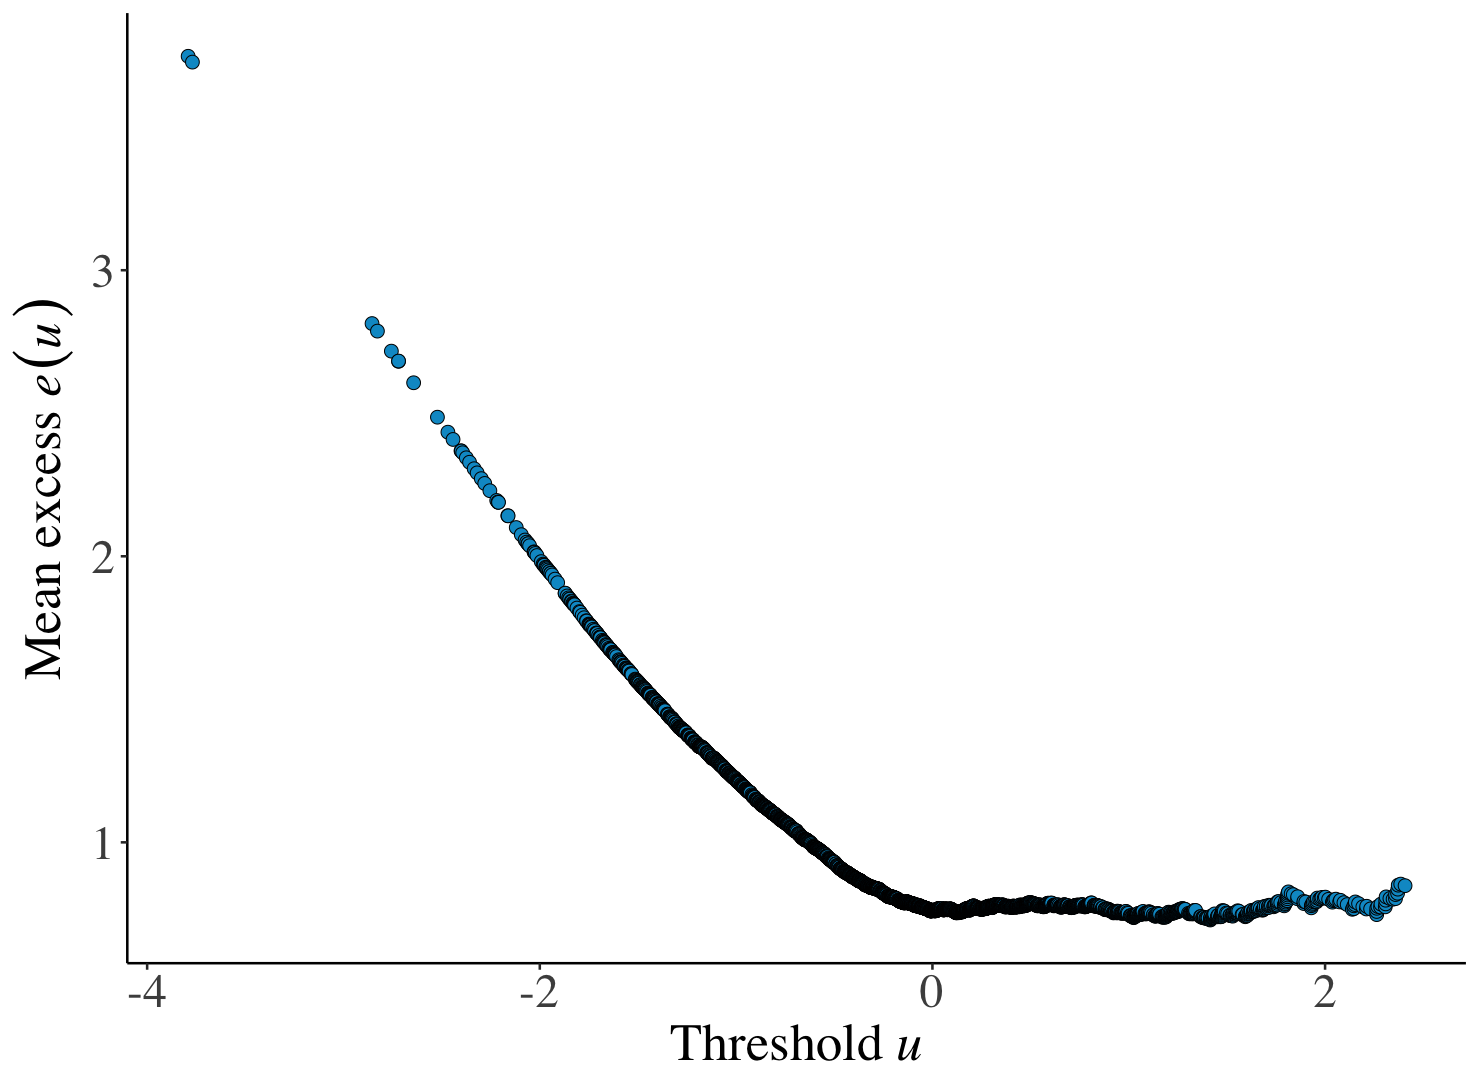
\includegraphics[width=0.95\linewidth]{3.11.png}
\column{0.49\textwidth}
\centering
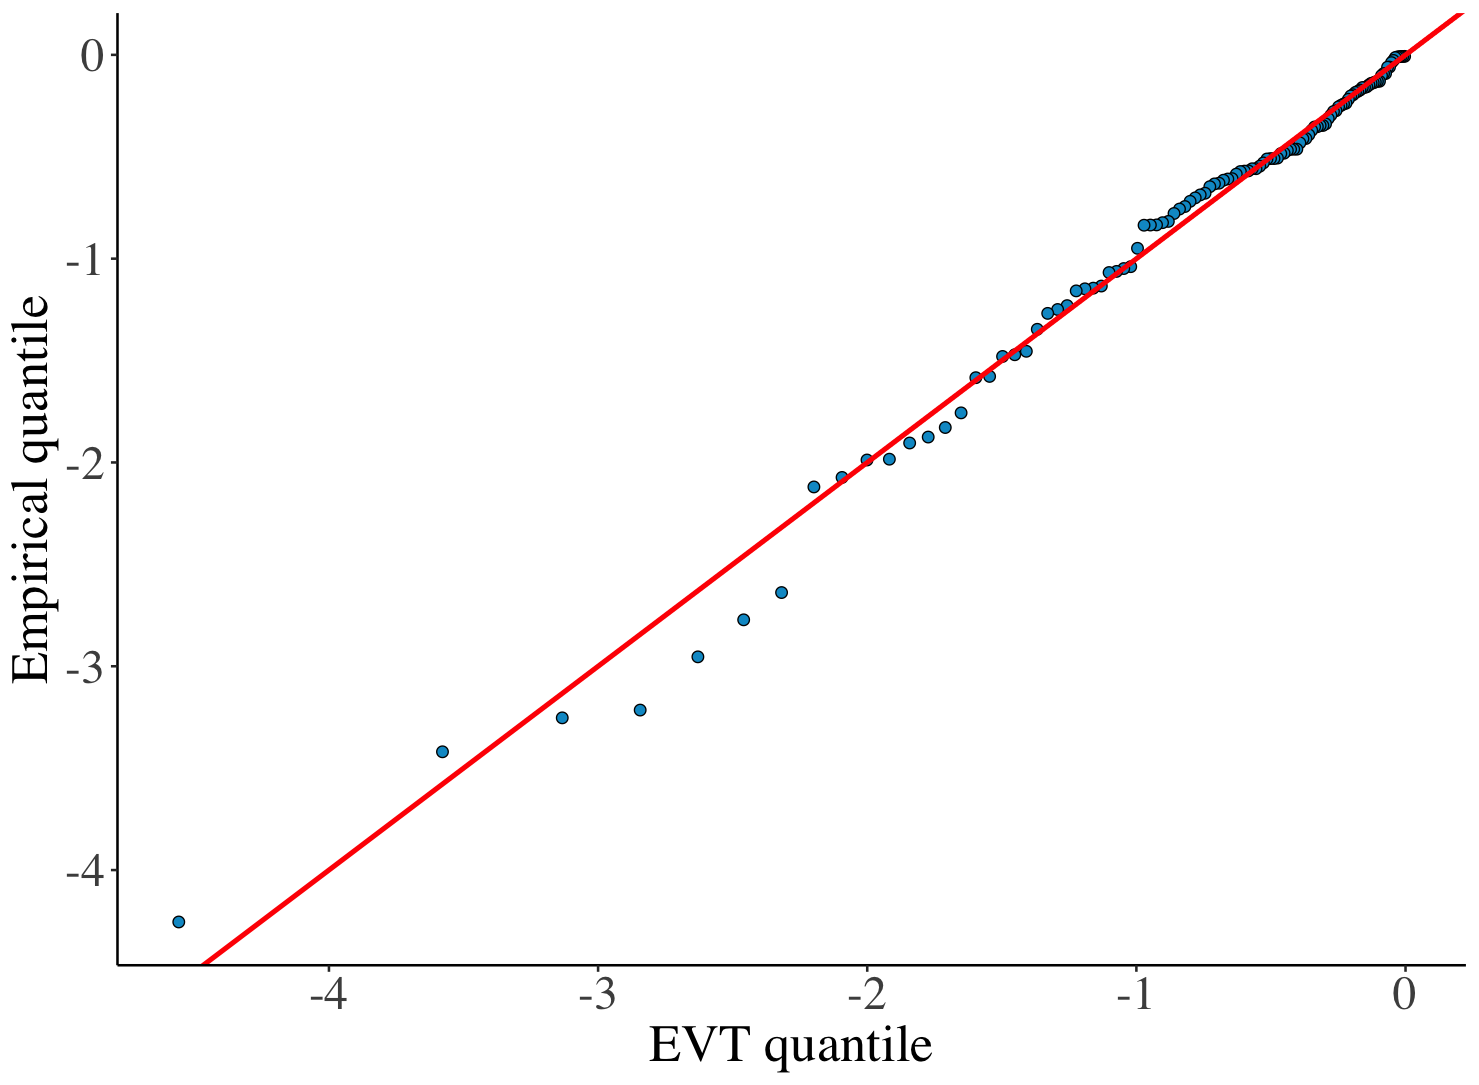
\includegraphics[width=0.95\linewidth]{3.13.png}
\end{columns}
\begin{itemize}
\item Mean excess plot supports \(u=1.8\).
\item GPD improves fit of the left tail versus full-distribution alternatives.
\end{itemize}
\end{frame}

\begin{frame}{Estimated Return Models}
\small
\begin{table}
\centering
\begin{tabular}{lcccc}
\toprule
Model & \(\alpha\) & \(\beta\) & \(\theta\) & Tail params \\
\midrule
GARCH-Asyt & 0.171 & 0.794 & -- & \(d_1=7.35,\ d_2=0.0115\) \\
GJR-Asyt & 0.054 & 0.795 & 4.62 & \(d_1=7.83,\ d_2=0.0129\) \\
GARCH-EVT & 0.171 & 0.794 & -- & \(\beta_{\text{GPD}}=0.774,\ \xi=0.029\) \\
GJR-EVT & 0.054 & 0.795 & 4.62 & \(\beta_{\text{GPD}}=0.621,\ \xi=0.206\) \\
\bottomrule
\end{tabular}
\end{table}
\begin{itemize}
\item Four complete univariate return models are ready for forecasting.
\end{itemize}
\end{frame}

\section{Forecasting and Evaluation}
\begin{frame}{Forecasting and Evaluation Framework}
\begin{itemize} \setlength{\itemsep}{1em}
\item Forecast horizon: 1 day ahead, test window Jan--Apr 2025.
\item Outputs: \(\sigma^2_{t+1}\), density forecast, VaR\(_{2.5\%}\), ES\(_{2.5\%}\).
\item Evaluation blocks:
\begin{itemize}
\item Volatility diagnostics (ACF of standardized squares, QLIKE, LR).
\item Risk diagnostics (Christoffersen \(LR_{\text{uc}}, LR_{\text{ind}}, LR_{\text{cc}}\)).
\item Density diagnostics (PIT histograms, KS , Berkowitz, DM).
\end{itemize}
\end{itemize}
\end{frame}

\begin{frame}{ACF of Standardized Squares}
\begin{columns}[T]
\column{0.49\textwidth}
\centering
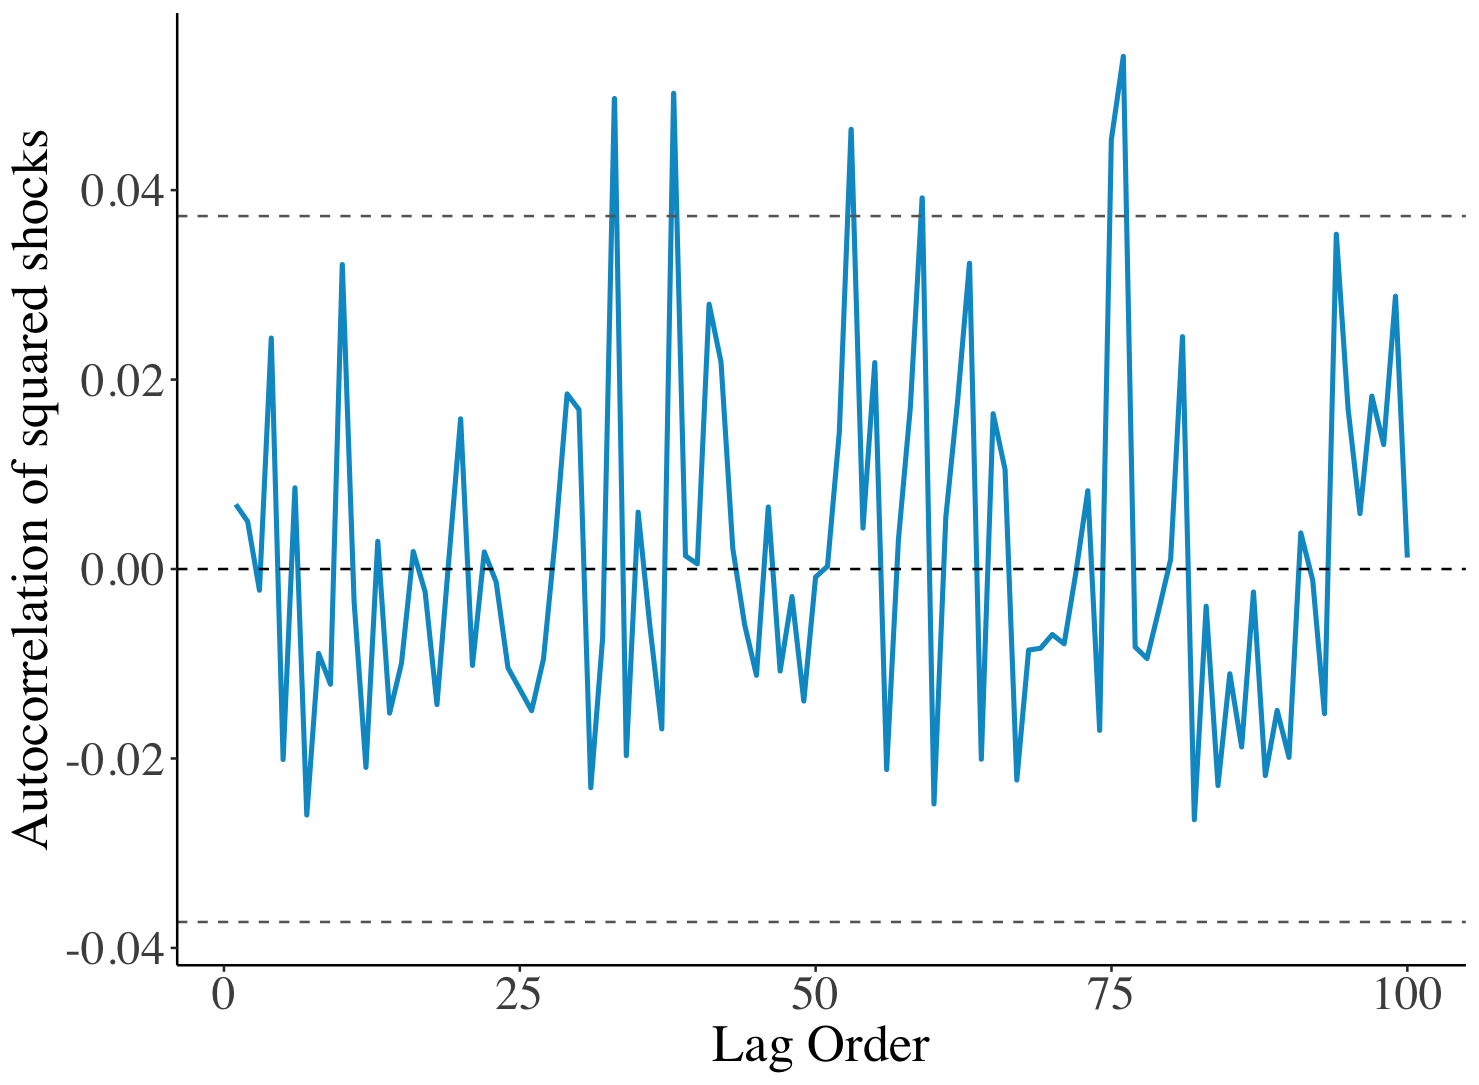
\includegraphics[width=0.95\linewidth]{4.1.png}
\vspace{0.1em}

\footnotesize GARCH(1,1)
\column{0.49\textwidth}
\centering
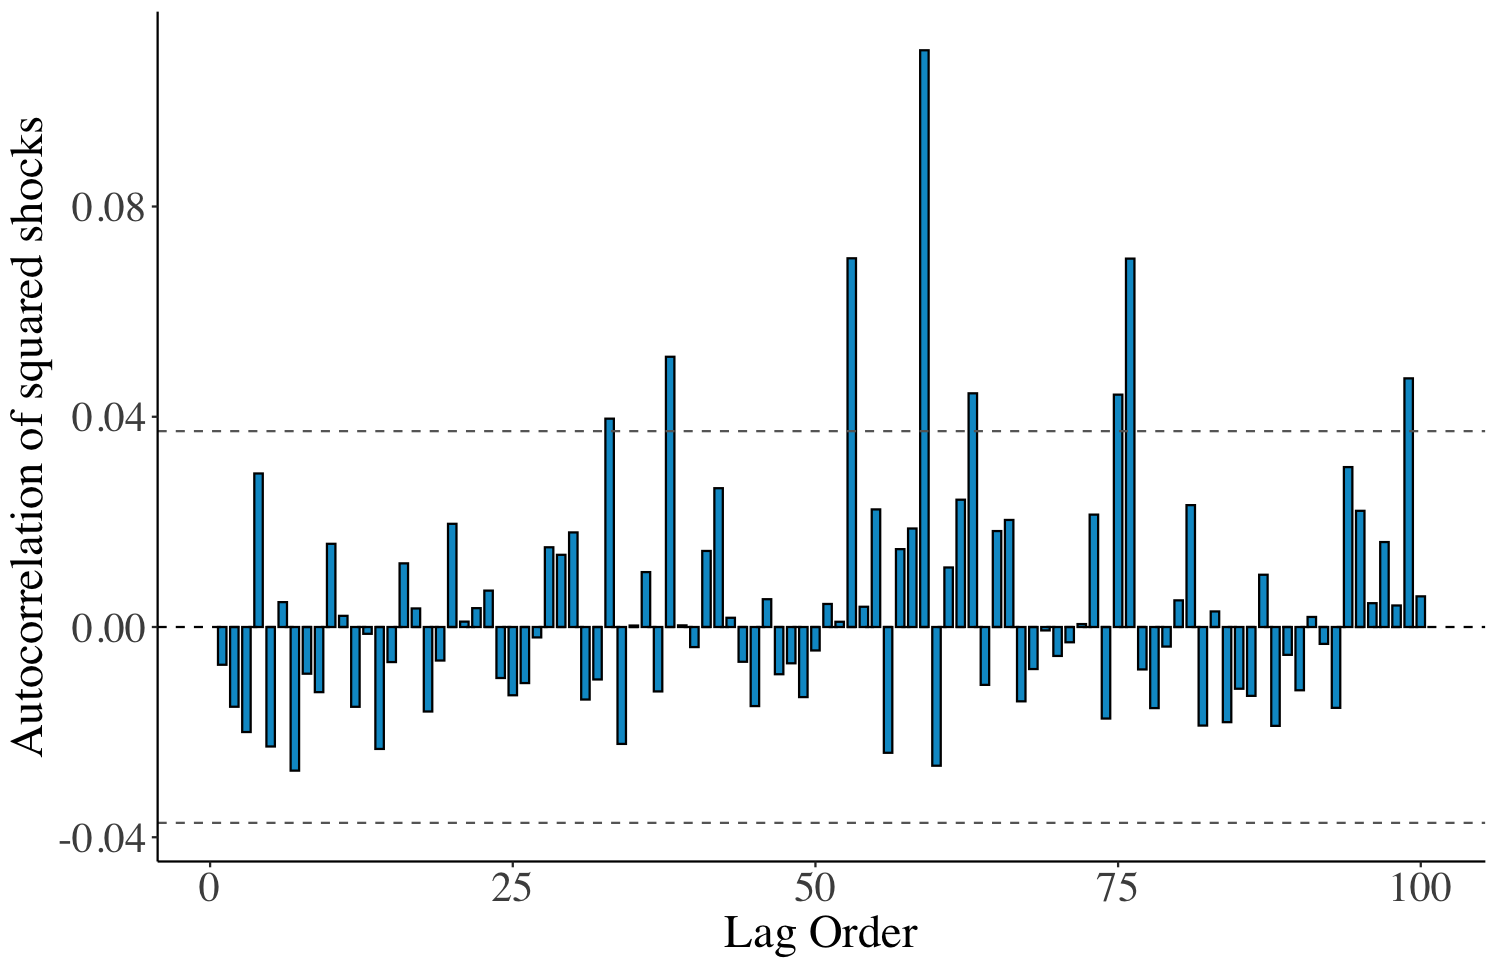
\includegraphics[width=0.95\linewidth]{4.2.png}
\vspace{0.1em}

\footnotesize GJR-GARCH(1,1)
\end{columns}
\begin{itemize}
\item Diagnostic goal: remove autocorrelation in standardized squared returns.
\item Both models substantially absorb the dependence structure.
\end{itemize}
\end{frame}

\begin{frame}{Asymmetric t Forecasts: VaR and ES}
\small
\[
\text{VaR}_{t+1}^{p}=-\sigma_{t+1}F^{-1}_{\text{asyt}}(p;d_1,d_2),\qquad
\text{ES}_{t+1}^{p}=-\sigma_{t+1}\text{ES}_{\text{asyt}}(p)
\]
\begin{itemize} \setlength{\itemsep}{1em}
\item Full-density models provide direct VaR and ES forecasts.
\item Calibration check at \(p=2.5\%\): expected violations about 2 in 81 days.
\end{itemize}
\end{frame}

\begin{frame}{Asymmetric t VaR Breaches (Test Period)}
\begin{columns}[T]
\column{0.49\textwidth}
\centering
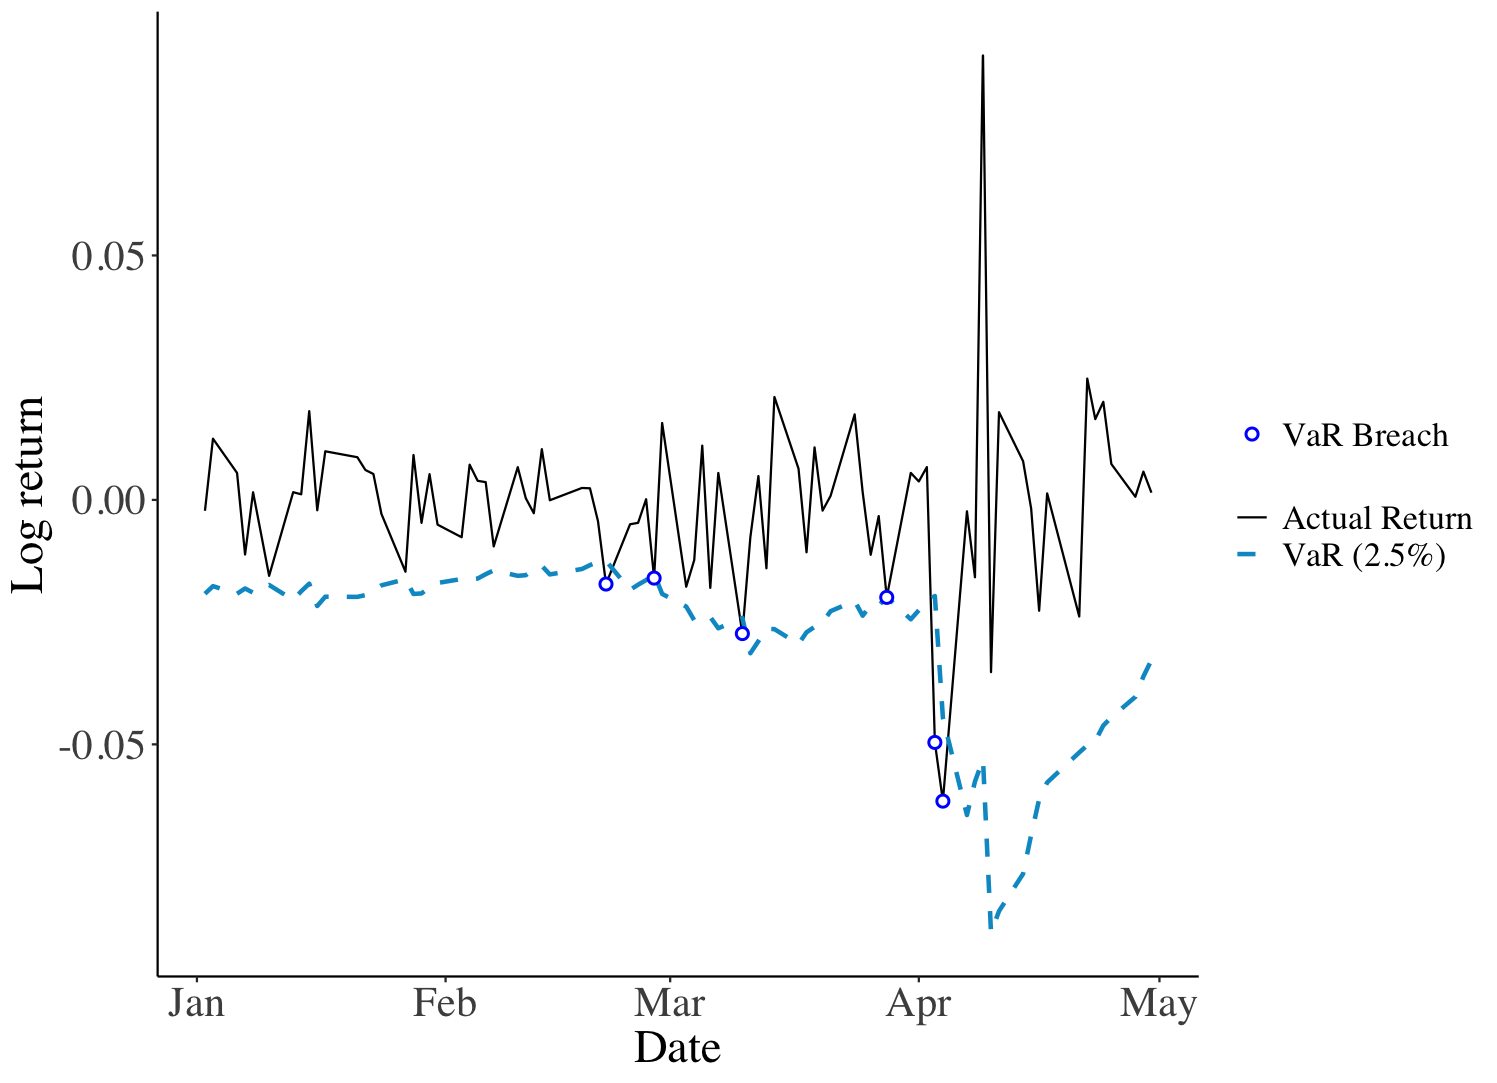
\includegraphics[width=0.95\linewidth]{4.3.png}
\column{0.49\textwidth}
\centering
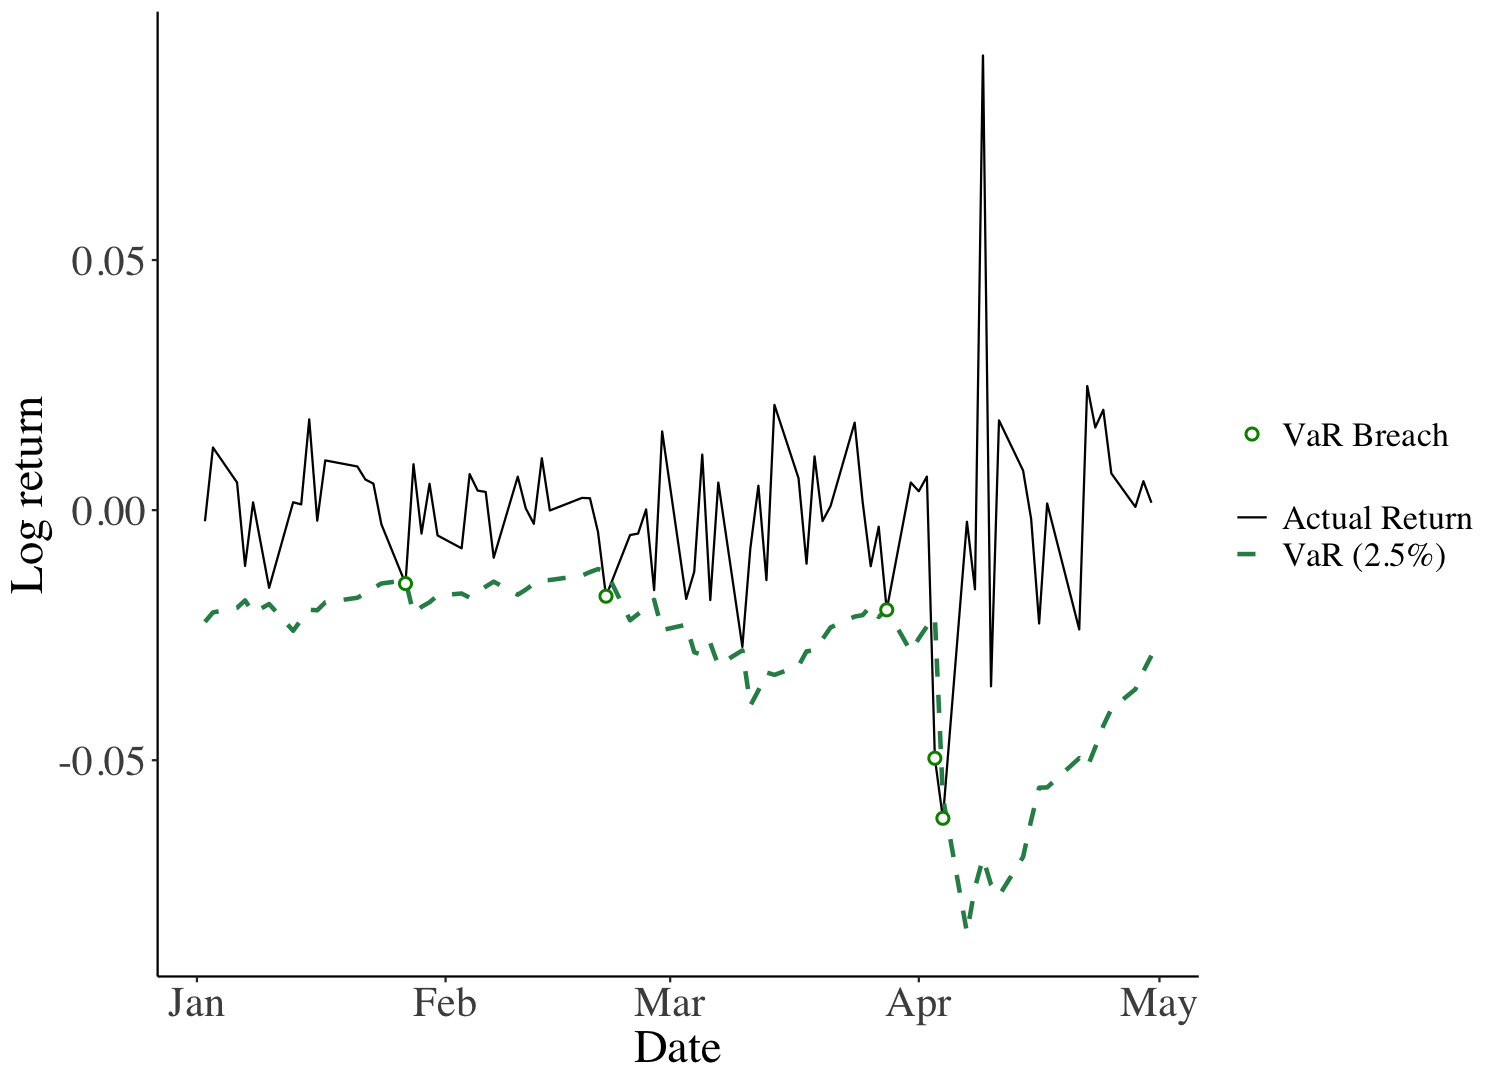
\includegraphics[width=0.95\linewidth]{4.4.png}
\end{columns}
\begin{itemize}
\item Observed breaches exceed expectation and cluster after volatility shock.
\end{itemize}
\end{frame}

\begin{frame}{Asymmetric t Backtesting (VaR)}
\begin{table}
\centering
\begin{tabular}{llcc}
\toprule
Test & p-value type & GARCH-Asyt & GJR-Asyt \\
\midrule
\(LR_{\text{uc}}\) & Simulated & 0.003 & 0.144 \\
\(LR_{\text{ind}}\) & Simulated & 0.095 & 0.047 \\
\(LR_{\text{cc}}\) & Simulated & 0.015 & 0.028 \\
\bottomrule
\end{tabular}
\end{table}
\begin{itemize} \setlength{\itemsep}{1em}
\item VaR performance is weak: coverage and independence issues.
\item Simulated \(LR_{\text{uc}}\) and \(LR_{\text{cc}}\) p-values are low for both models.
\item Breaches cluster around volatility jumps, violating independence.
\end{itemize}
\end{frame}

\begin{frame}{Asymmetric t Density Checks}
\begin{columns}[T]
\column{0.49\textwidth}
\centering
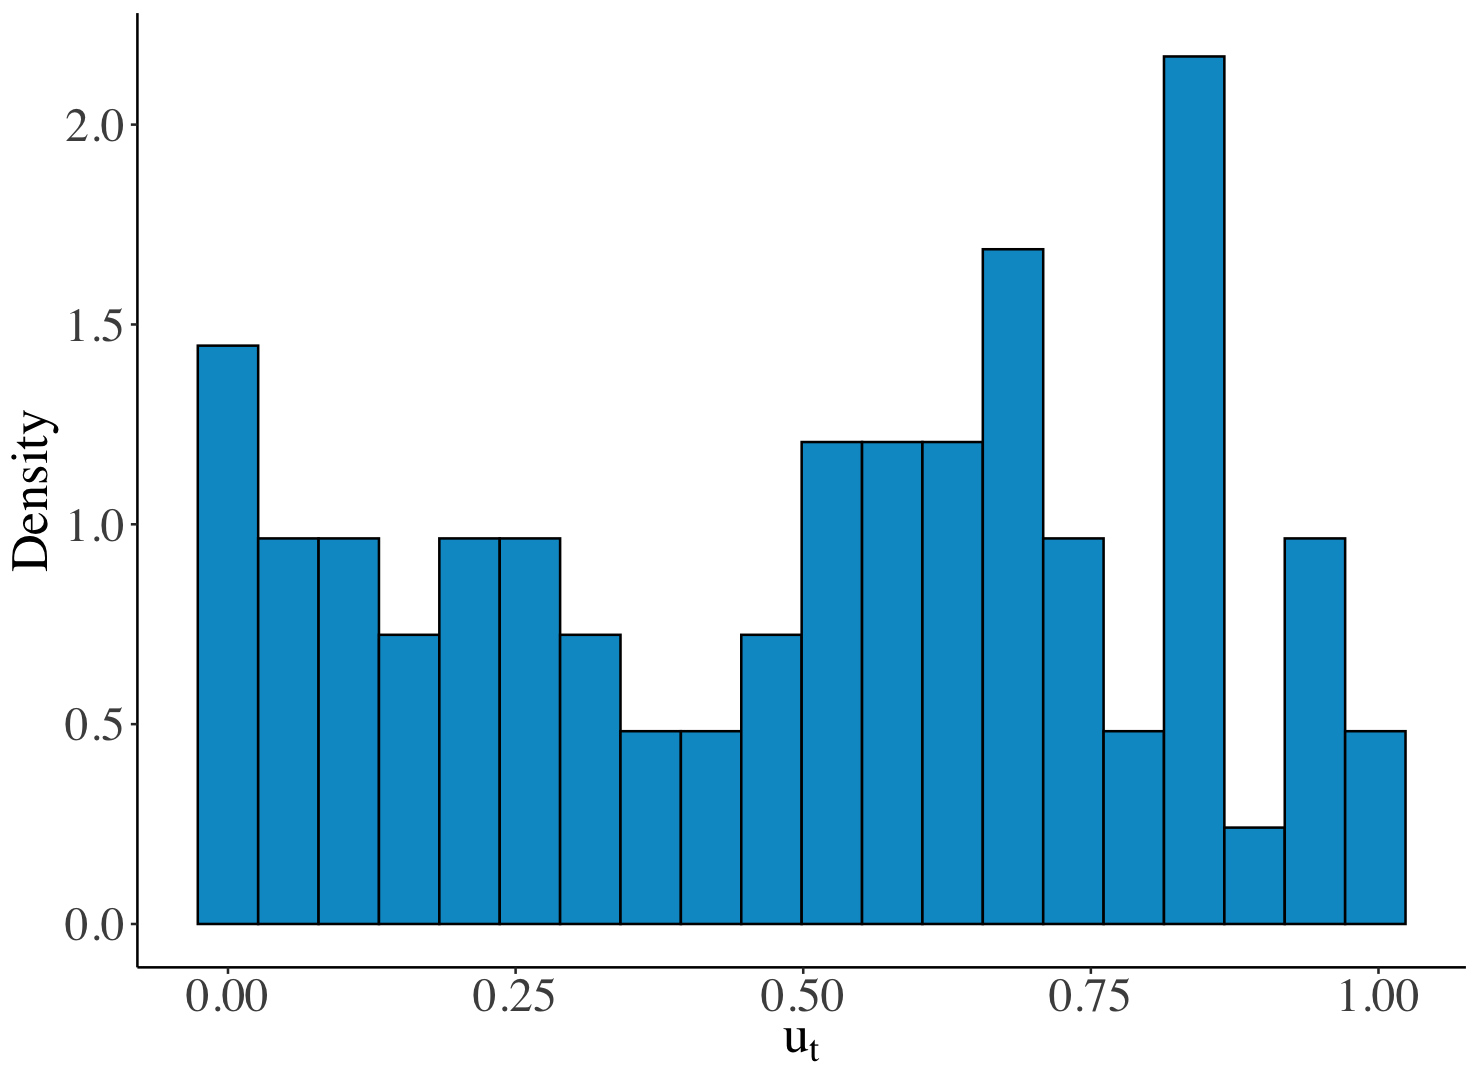
\includegraphics[width=0.95\linewidth]{4.7.png}
\vspace{0.1em}

\footnotesize PIT histogram (GARCH-Asyt)
\column{0.49\textwidth}
\centering
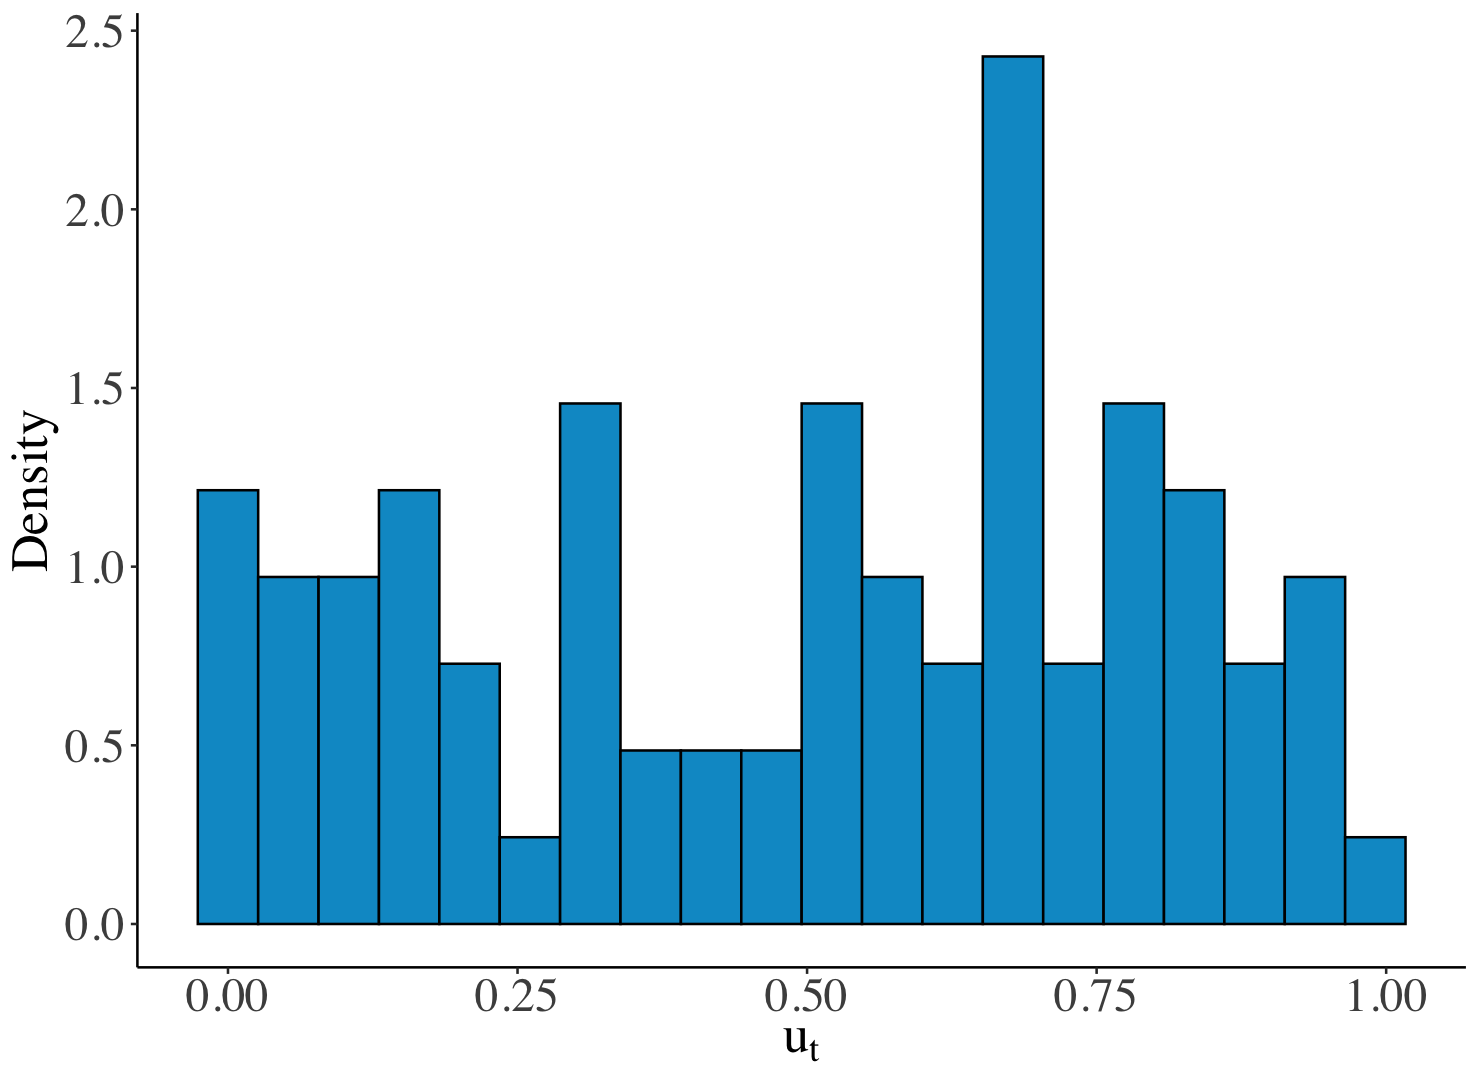
\includegraphics[width=0.95\linewidth]{4.8.png}
\vspace{0.1em}

\footnotesize PIT histogram (GJR-Asyt)
\end{columns}
\begin{itemize}
\item KS on \(\Phi^{-1}(u_{t+1})\): 0.8512 (GARCH-Asyt), 0.7931 (GJR-Asyt).
\item DM comparison: \(p=0.015\), favoring GJR-Asyt density forecasts.
\end{itemize}
\end{frame}

\begin{frame}{EVT Forecasts in the Test Period}
\begin{columns}[T]
\column{0.49\textwidth}
\centering
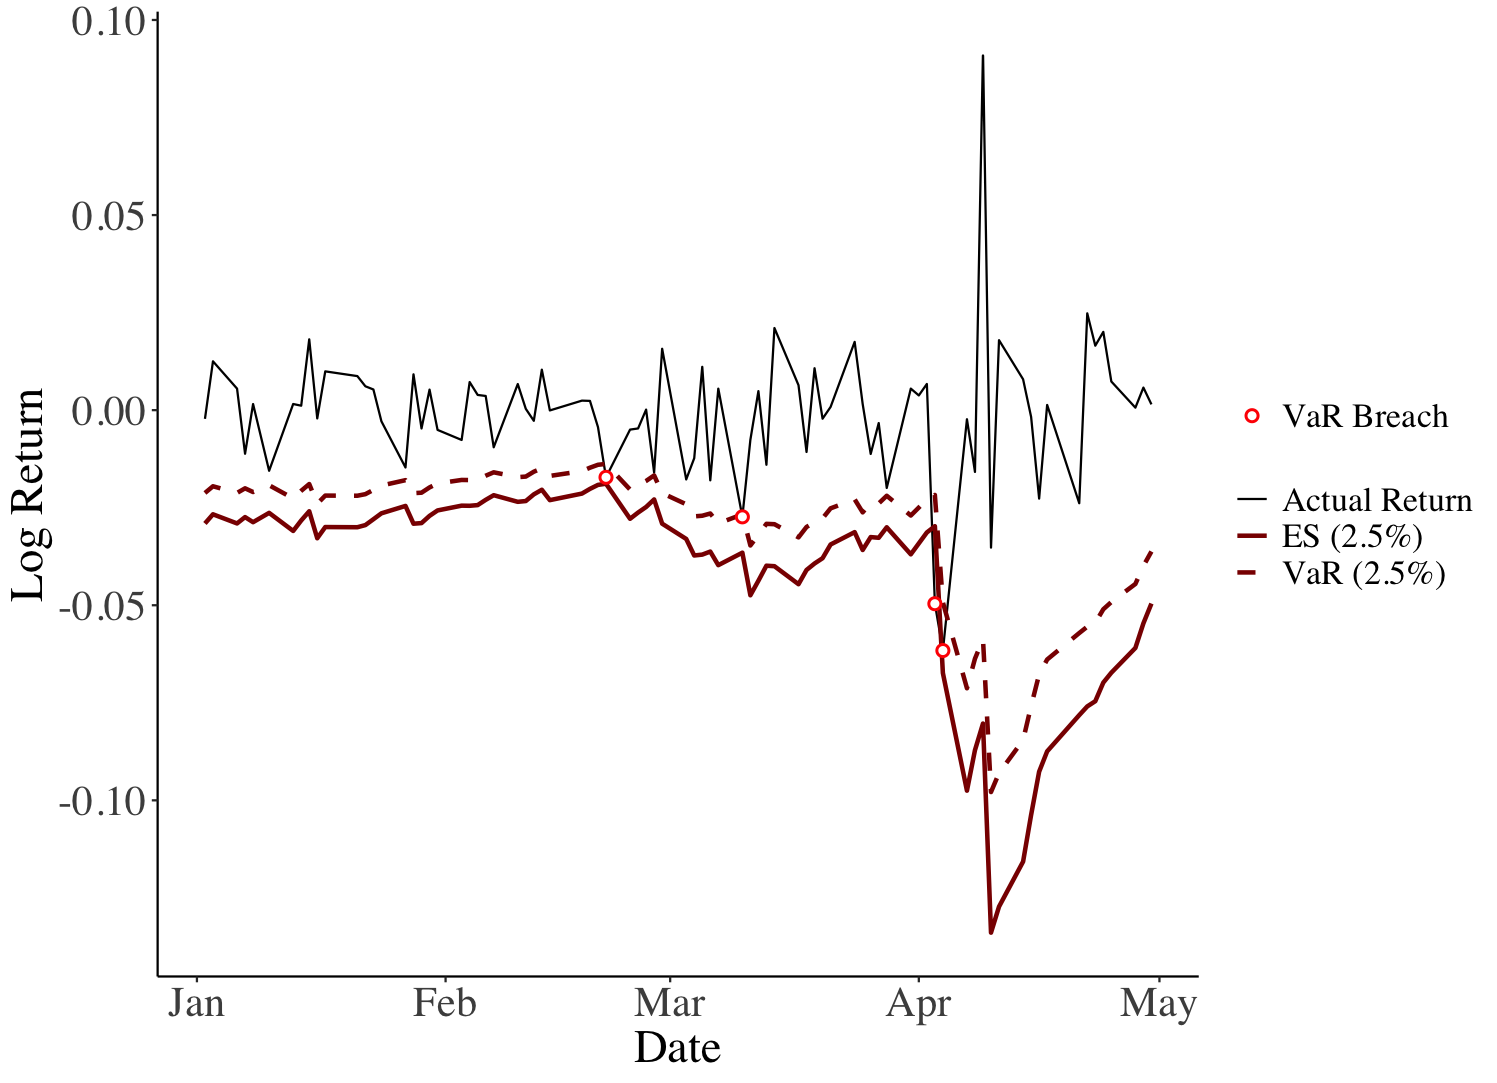
\includegraphics[width=0.95\linewidth]{4.11.png}
\column{0.49\textwidth}
\centering
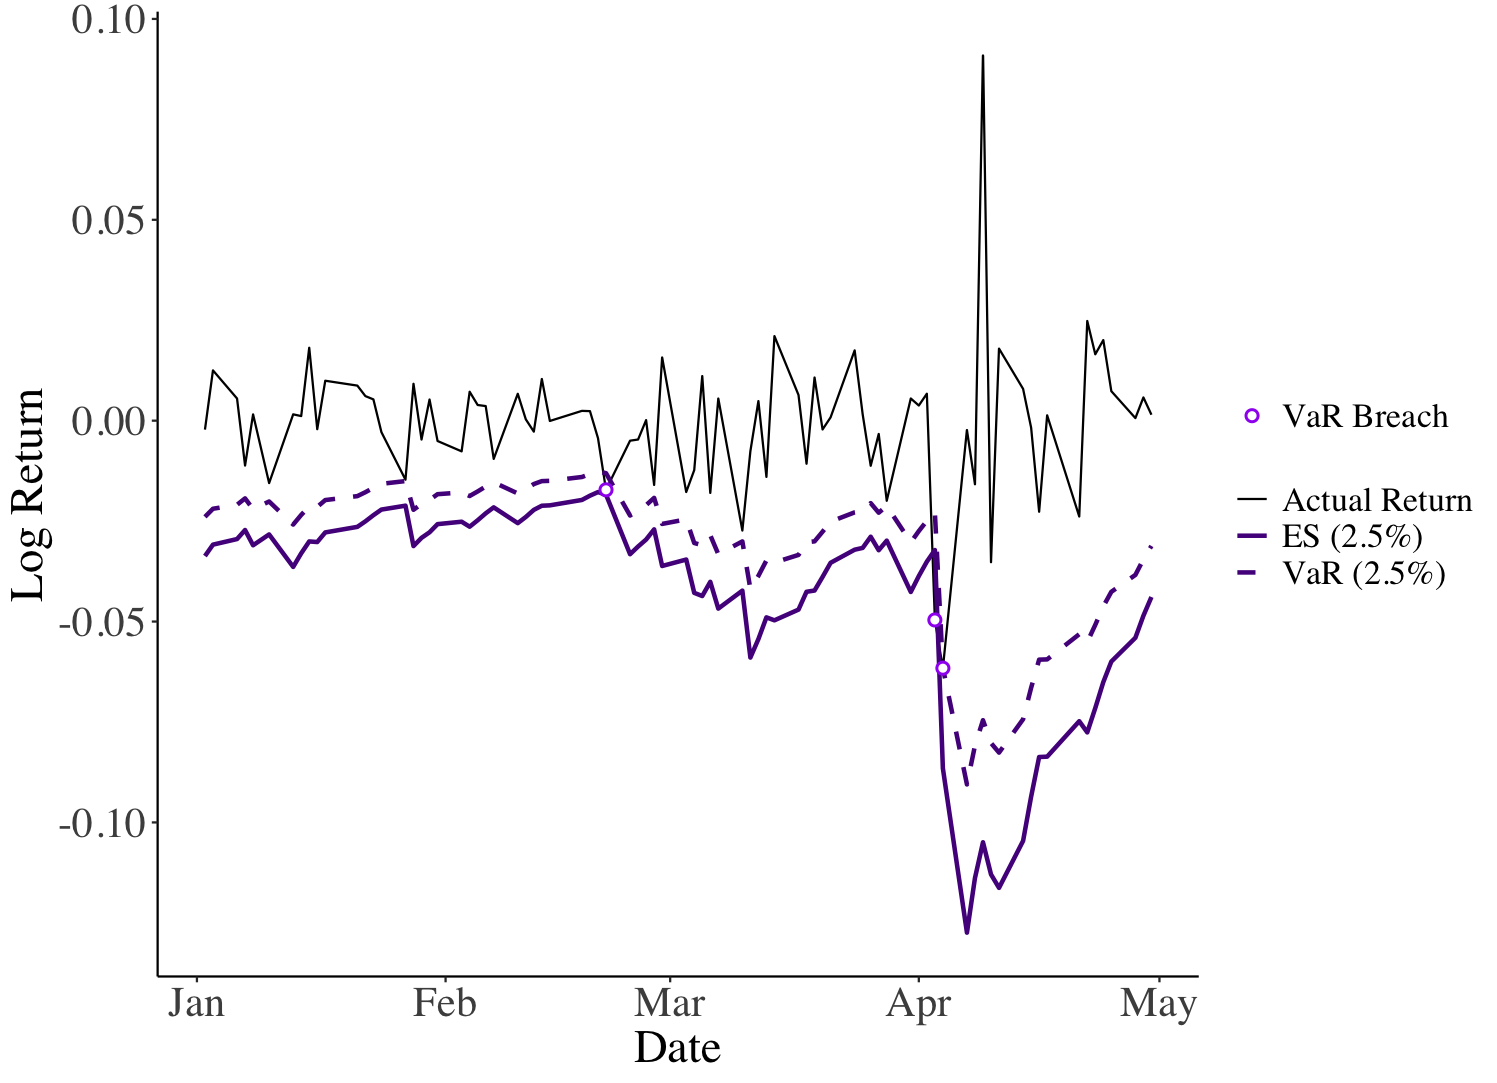
\includegraphics[width=0.95\linewidth]{4.12.png}
\end{columns}
\begin{itemize}
\item EVT focuses directly on the left tail, giving more conservative risk forecasts.
\item EVT variants show fewer breaches than Asyt counterparts.
\end{itemize}
\end{frame}

\begin{frame}{EVT Backtesting Summary}
\begin{table}
\centering
\begin{tabular}{llcc}
\toprule
Test & p-value type & GARCH-EVT & GJR-EVT \\
\midrule
\(LR_{\text{uc}}\) & Simulated & 0.188 & 0.554 \\
\(LR_{\text{ind}}\) & Simulated & 0.030 & 0.013 \\
\(LR_{\text{cc}}\) & Simulated & 0.217 & 0.200 \\
\bottomrule
\end{tabular}
\end{table}
\begin{itemize} \setlength{\itemsep}{1em}
\item Coverage improves, but independence of violations remains problematic.
\item Main weakness: slow adaptation to abrupt volatility regime changes.
\item Stress-testing (2008 episode) supports stronger breach control for EVT variants.
\end{itemize}
\end{frame}

\section{Copula Multivariate Model}
\begin{frame}{Why Copulas?}
\begin{columns}[T]
\column{0.49\textwidth}
\centering
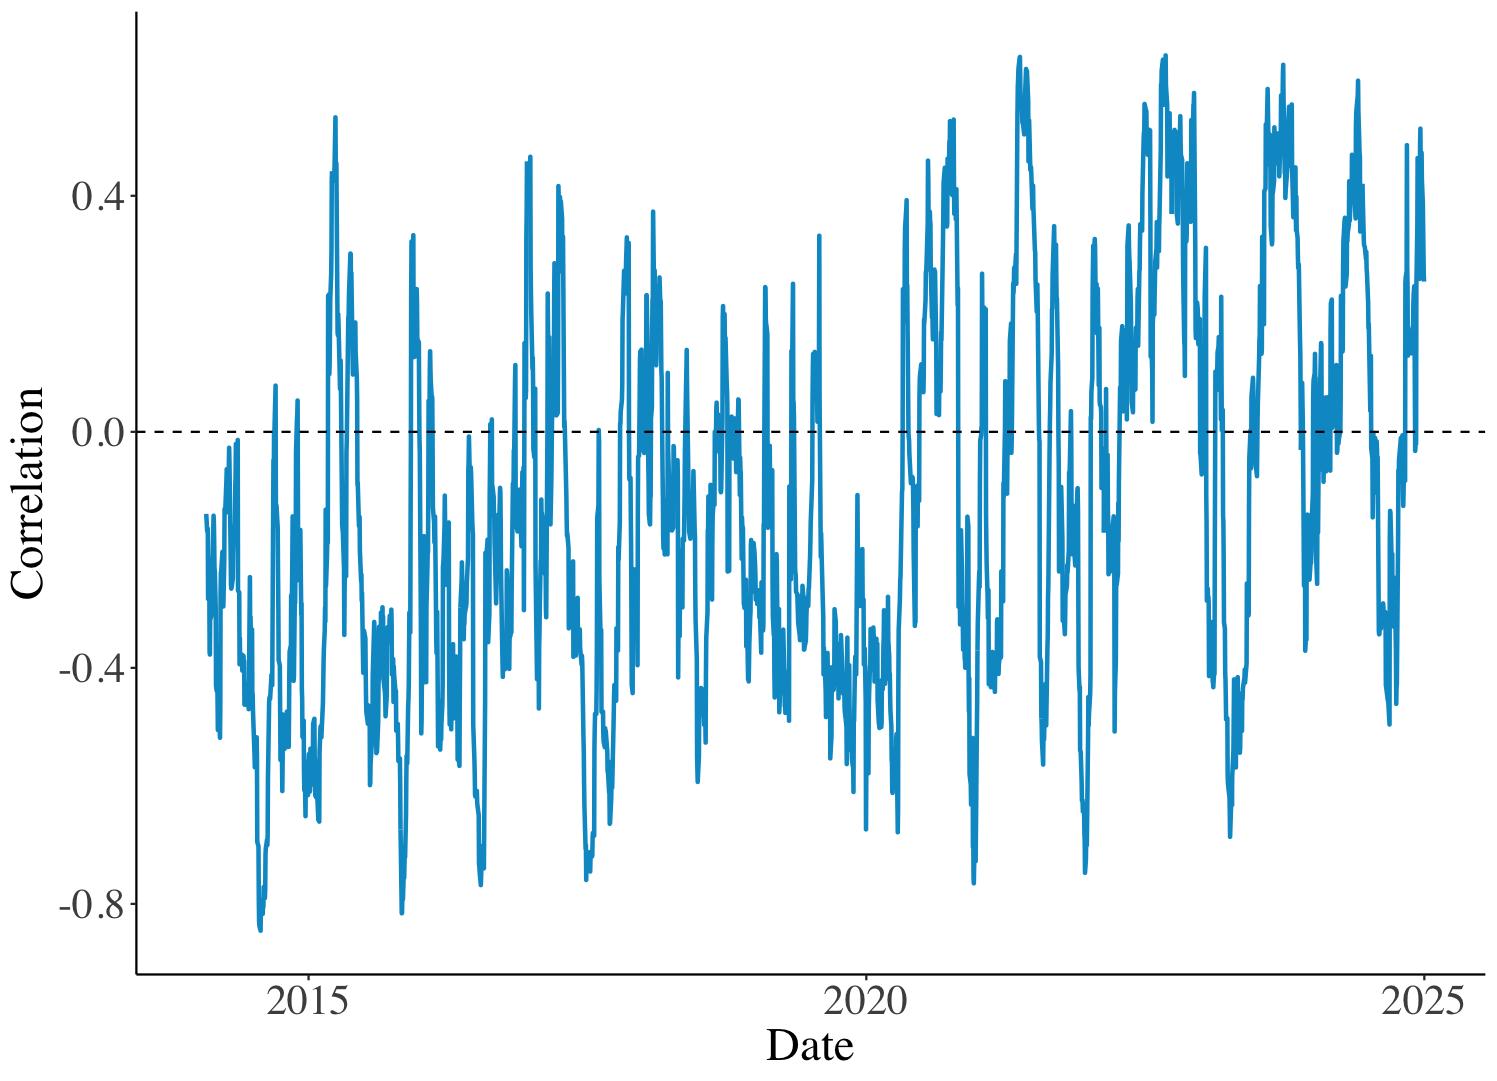
\includegraphics[width=\linewidth]{5.1.png}
\column{0.49\textwidth}
\centering
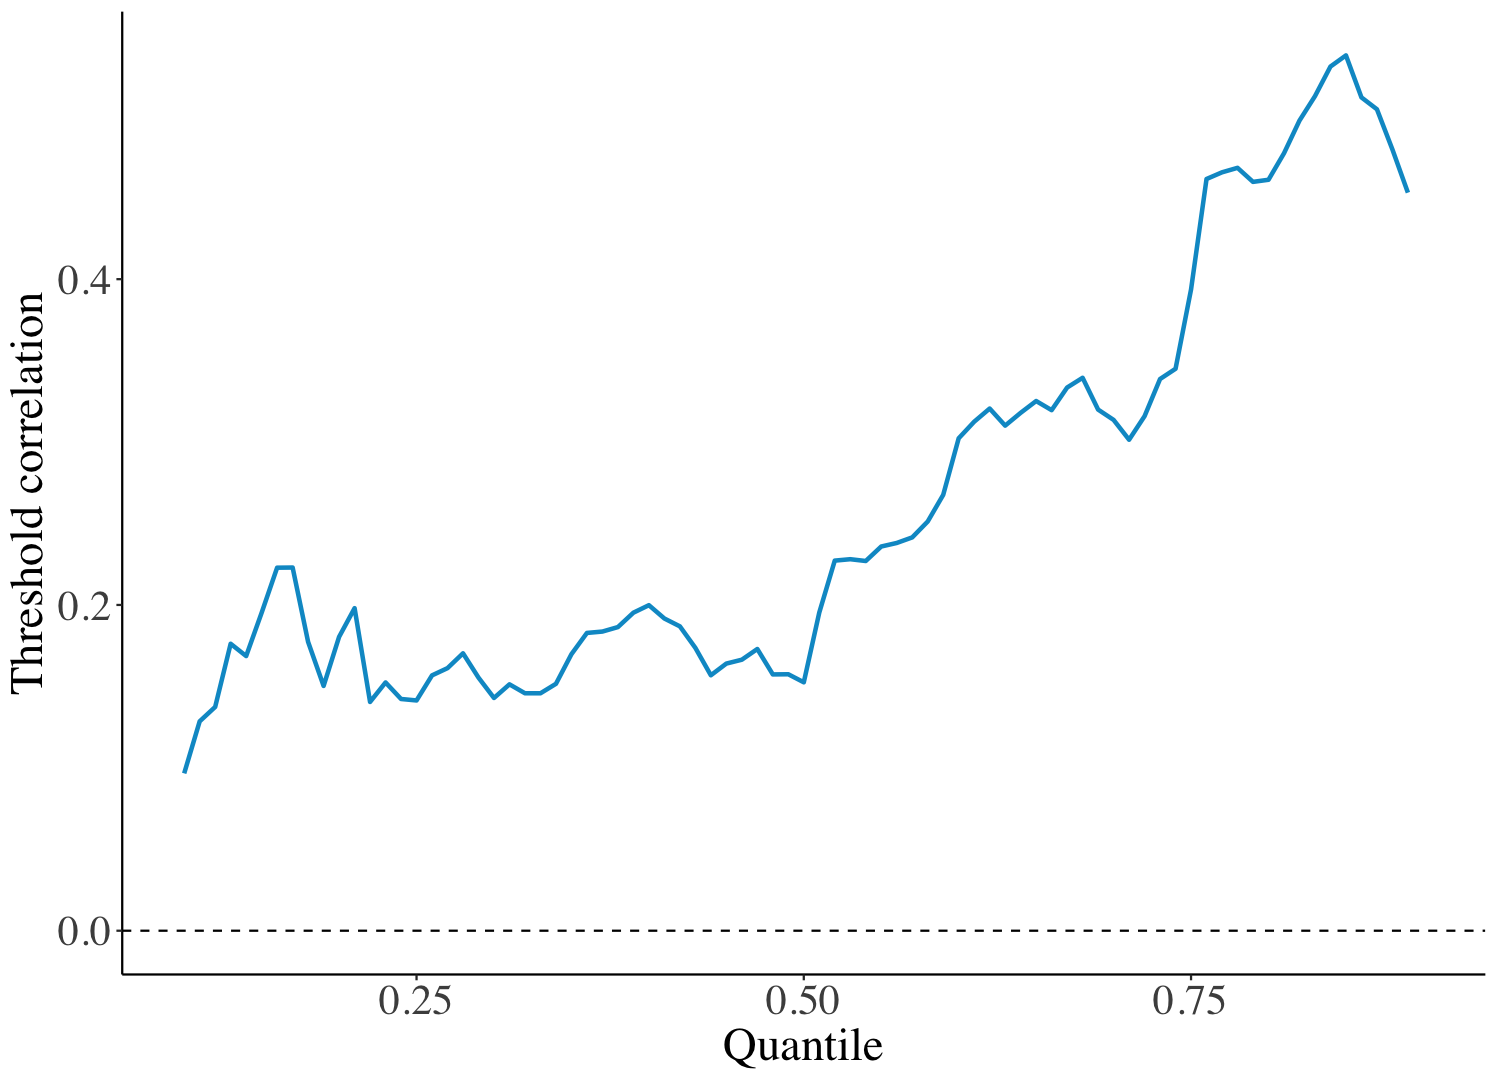
\includegraphics[width=\linewidth]{5.2.png}
\end{columns}
\begin{itemize}
\item Need dependence modeling for active risk management and diversification analysis.
\item DCC captures dynamic linear dependence; copulas also target nonlinear tail dependence.
\item Threshold-correlation evidence motivates copula-based modeling.
\end{itemize}
\end{frame}

\begin{frame}{t-Copula Specification and Estimation}
\[
G(u_1,u_2;\rho^*,d)=t_{(d,\rho^*)}\!\left(t^{-1}(u_1;d),t^{-1}(u_2;d)\right)
\]
\begin{table}
\centering
\begin{tabular}{lcc}
\toprule
Copula model & \(\rho^*\) & \(d\) \\
\midrule
GARCH-GARCH & -0.2121 & 4.9671 \\
GJR-GJR & -0.2088 & 4.8304 \\
\bottomrule
\end{tabular}
\end{table}
\begin{itemize} \setlength{\itemsep}{1em}
\item Static t-copula chosen for tractability and tail-thickness flexibility.
\item Marginals estimated first (GARCH-Asyt / GJR-Asyt), then copula parameters.
\end{itemize}
\end{frame}

\begin{frame}{Threshold-Correlation Fit}
\begin{columns}[T]
\column{0.49\textwidth}
\centering
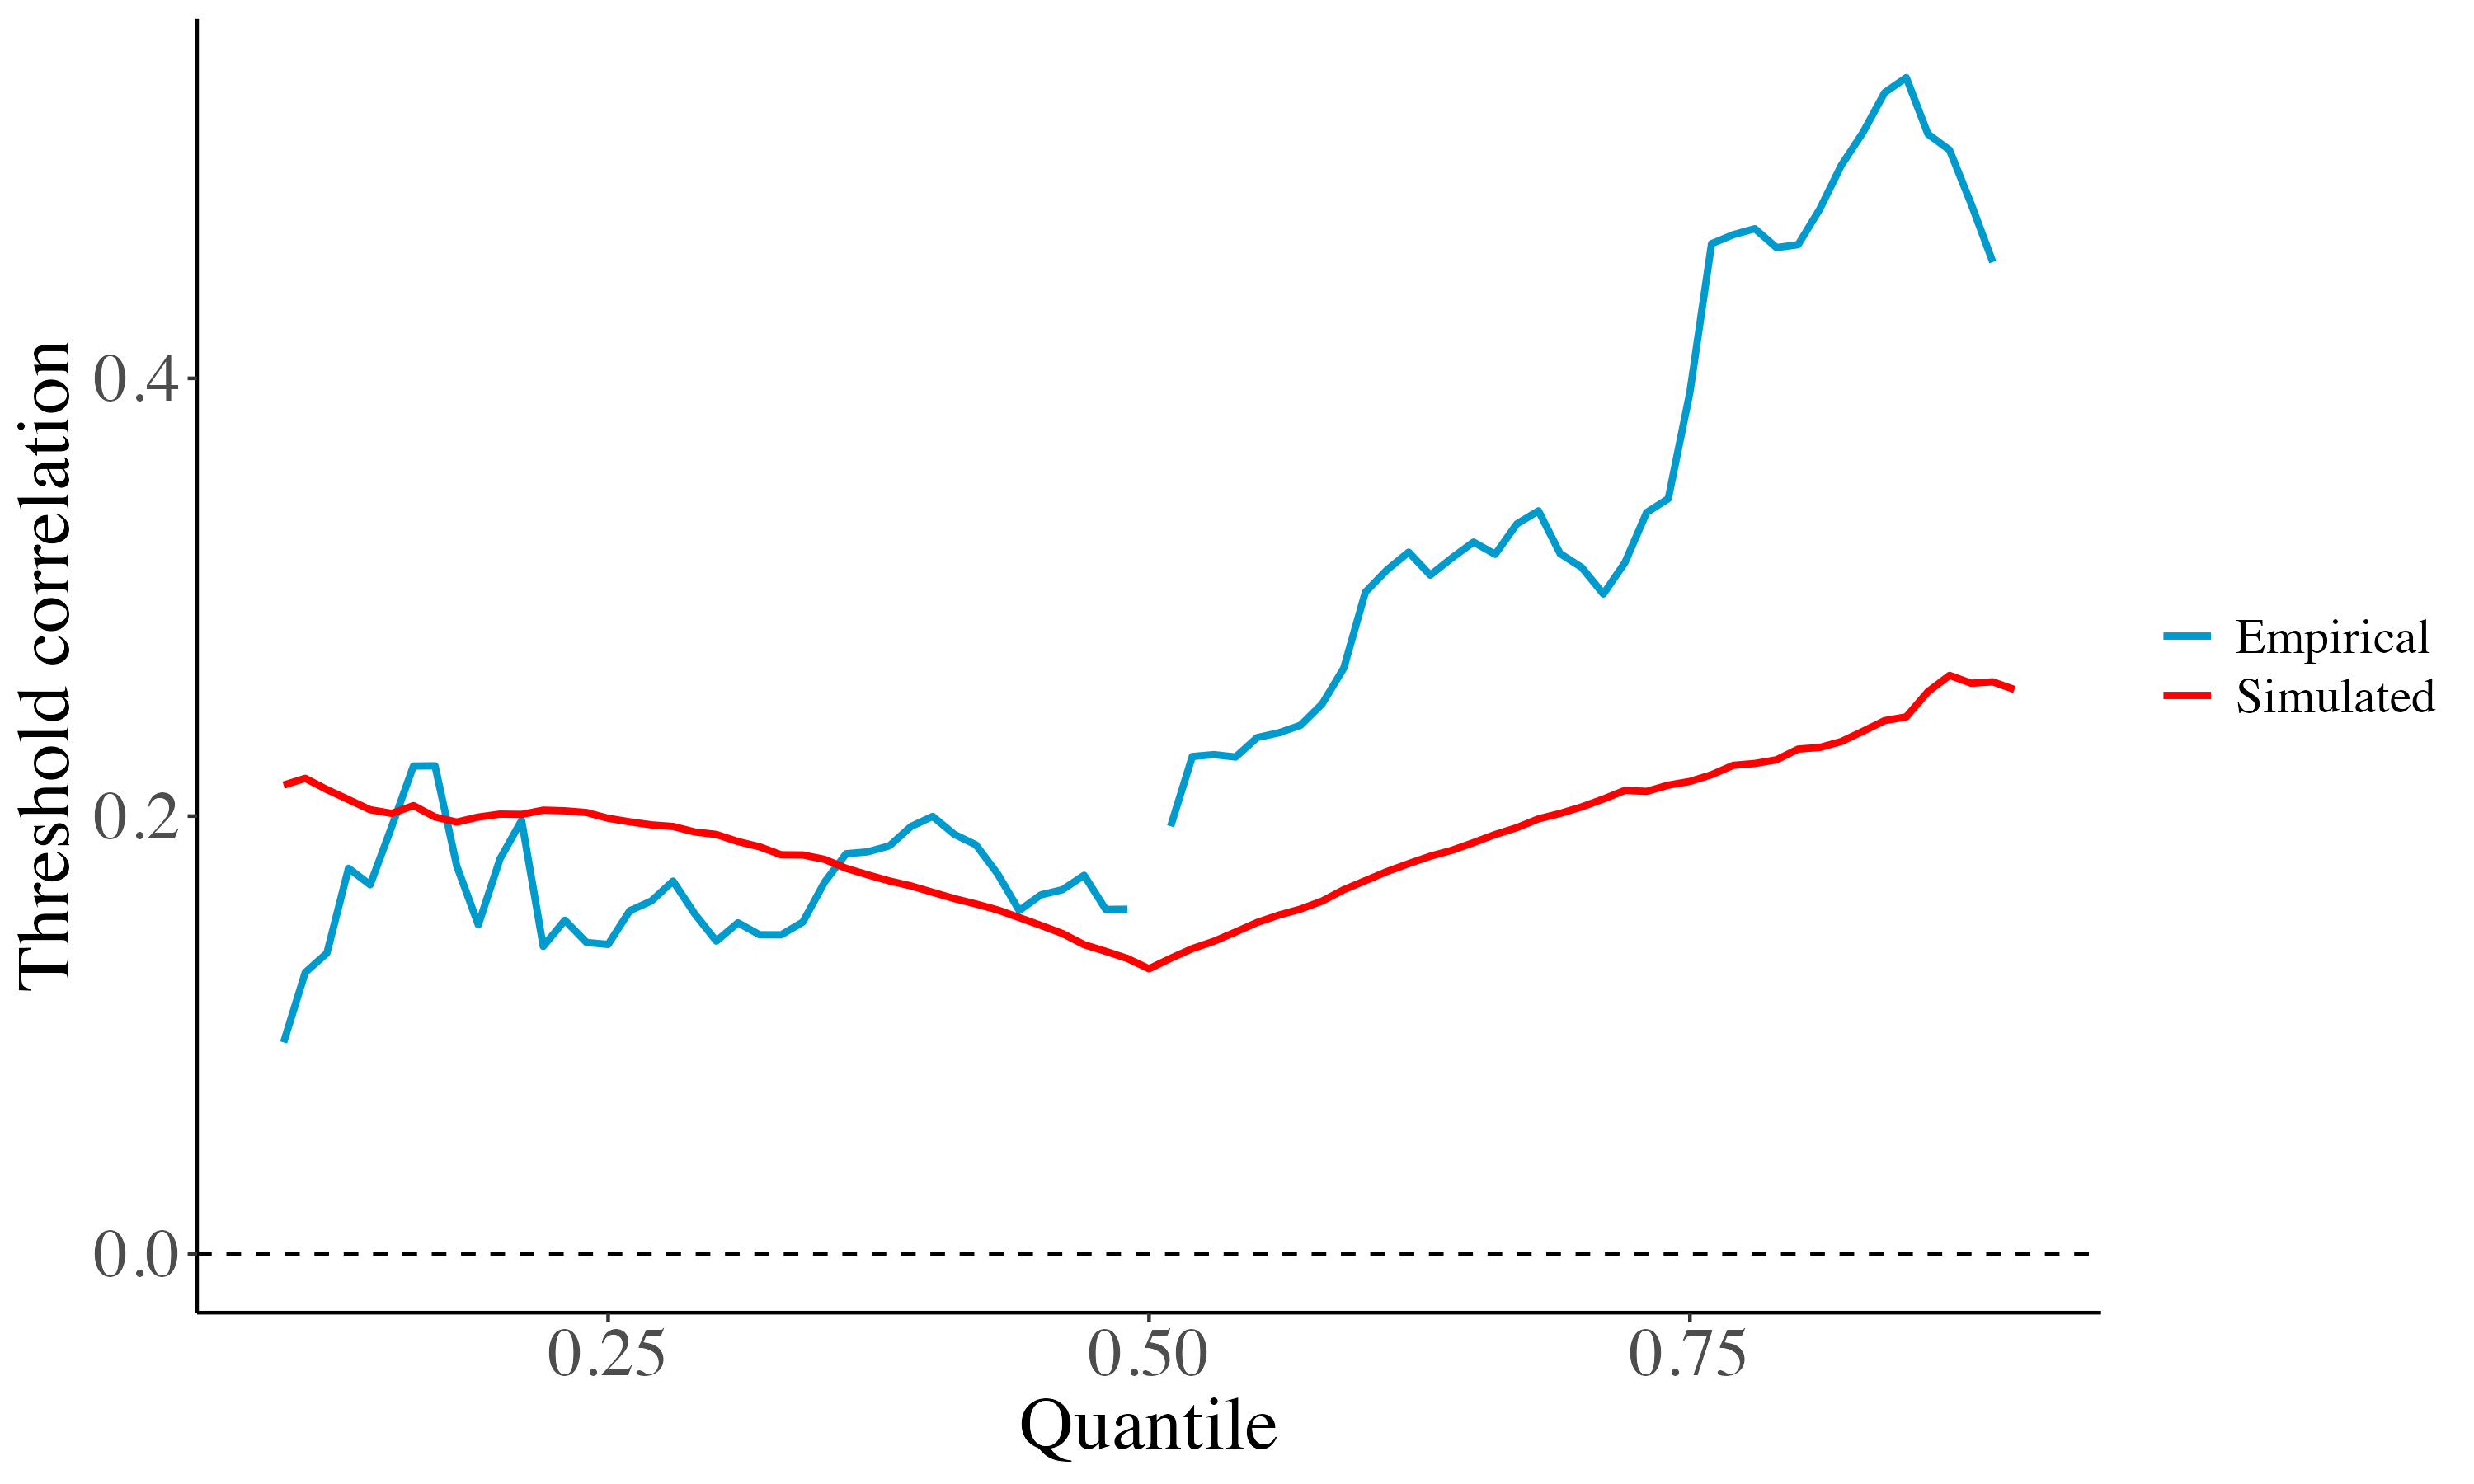
\includegraphics[width=0.95\linewidth]{5.3.png}
\vspace{0.1em}

\footnotesize GARCH-GARCH copula
\column{0.49\textwidth}
\centering
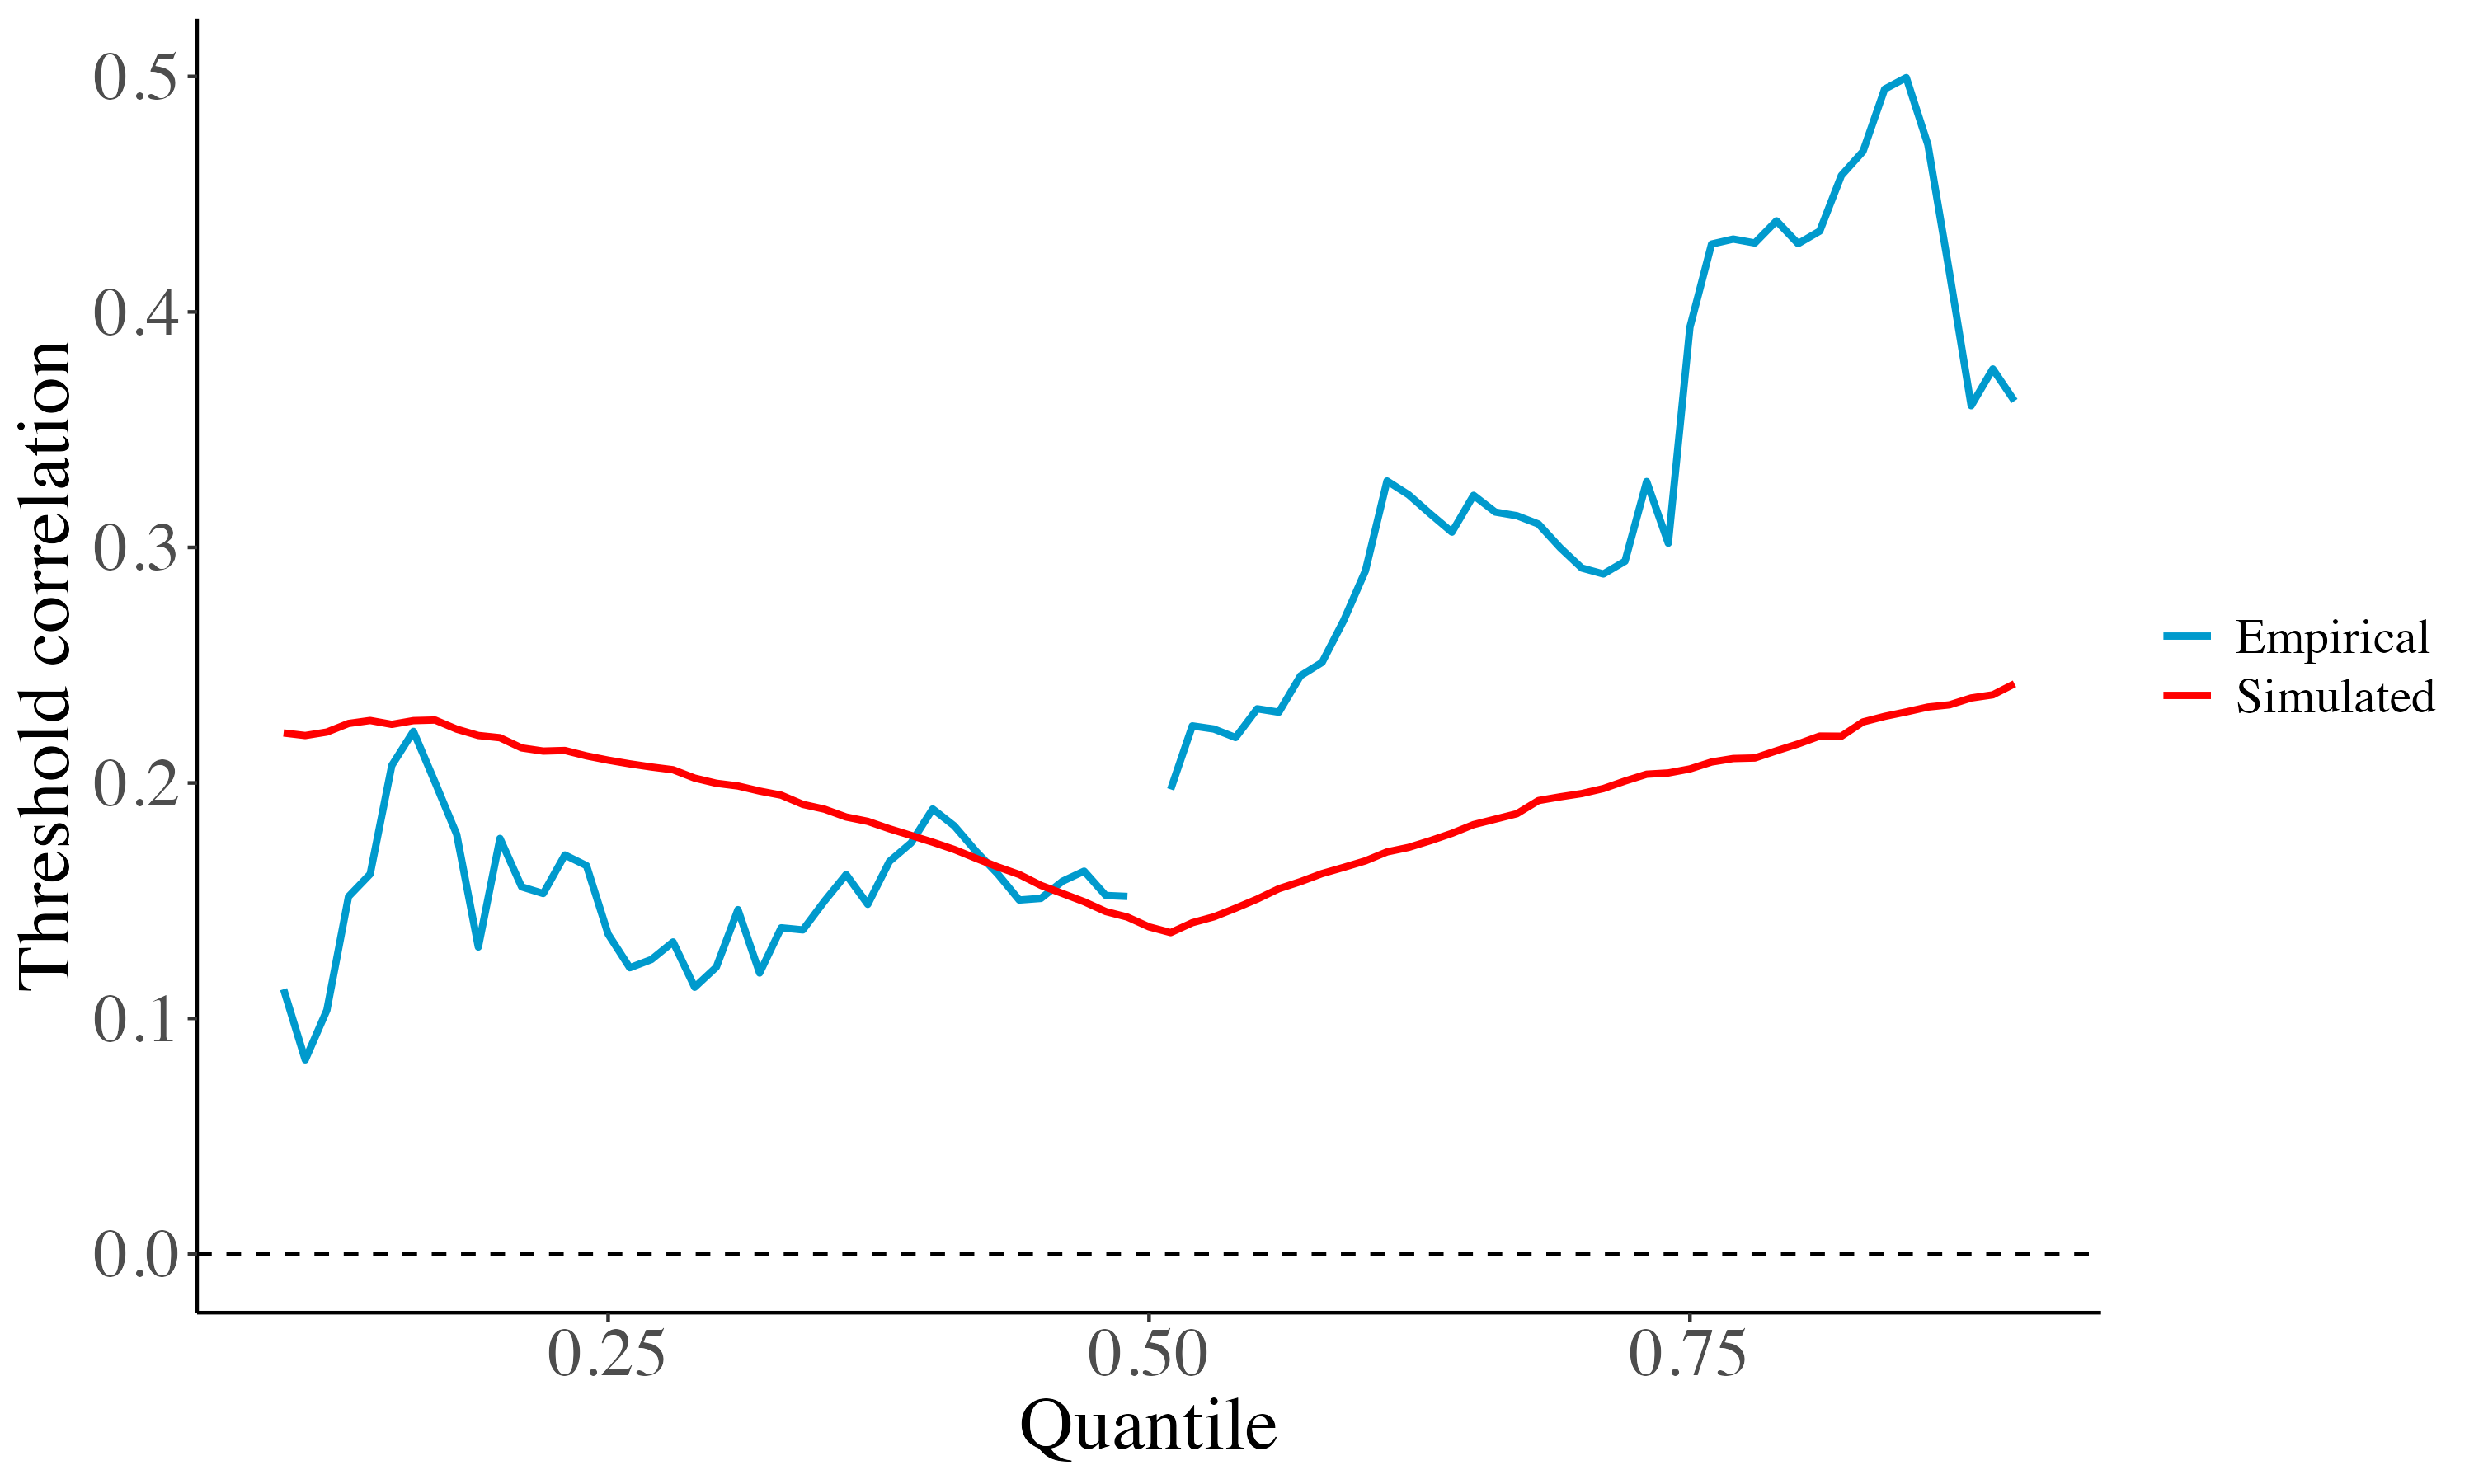
\includegraphics[width=0.95\linewidth]{5.4.png}
\vspace{0.1em}

\footnotesize GJR-GJR copula
\end{columns}
\begin{itemize}
\item t-copula reproduces heavier dependence in both tails reasonably well.
\item Right-tail asymmetry in data is only partially captured (copula is symmetric).
\end{itemize}
\end{frame}

\begin{frame}{Monte Carlo Forecasting Pipeline}
\begin{center}
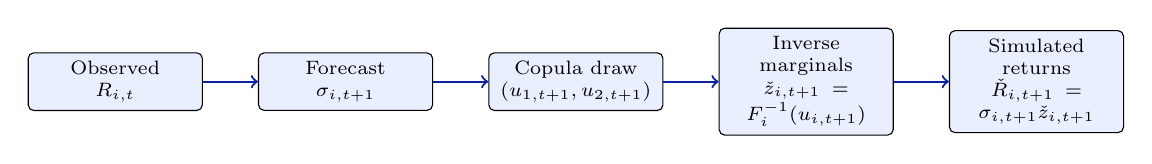
\begin{tikzpicture}[
  node distance=0.9cm and 0.7cm,
  pipeline/.style={draw, rounded corners=2pt, fill=itamlight, align=center, inner sep=3pt, text width=2.0cm, font=\scriptsize},
  arrow/.style={->, thick, color=itamblue}
]
\node[pipeline] (r) {Observed\\\(R_{i,t}\)};
\node[pipeline,right=of r] (sig) {Forecast\\\(\sigma_{i,t+1}\)};
\node[pipeline,right=of sig] (u) {Copula draw\\\((u_{1,t+1},u_{2,t+1})\)};
\node[pipeline,right=of u] (z) {Inverse marginals\\\(\check z_{i,t+1}=F_i^{-1}(u_{i,t+1})\)};
\node[pipeline,right=of z] (rp) {Simulated returns\\\(\check R_{i,t+1}=\sigma_{i,t+1}\check z_{i,t+1}\)};
\draw[arrow] (r) -- (sig);
\draw[arrow] (sig) -- (u);
\draw[arrow] (u) -- (z);
\draw[arrow] (z) -- (rp);
\end{tikzpicture}
\end{center}
\begin{itemize} \setlength{\itemsep}{1em}
\item Repeat \(M\) times to form portfolio-return density.
\item Compute VaR/ES from simulated quantiles and tail means.
\end{itemize}
\end{frame}

\begin{frame}{Copula Portfolio Results}
\begin{columns}[T]
\column{0.49\textwidth}
\centering
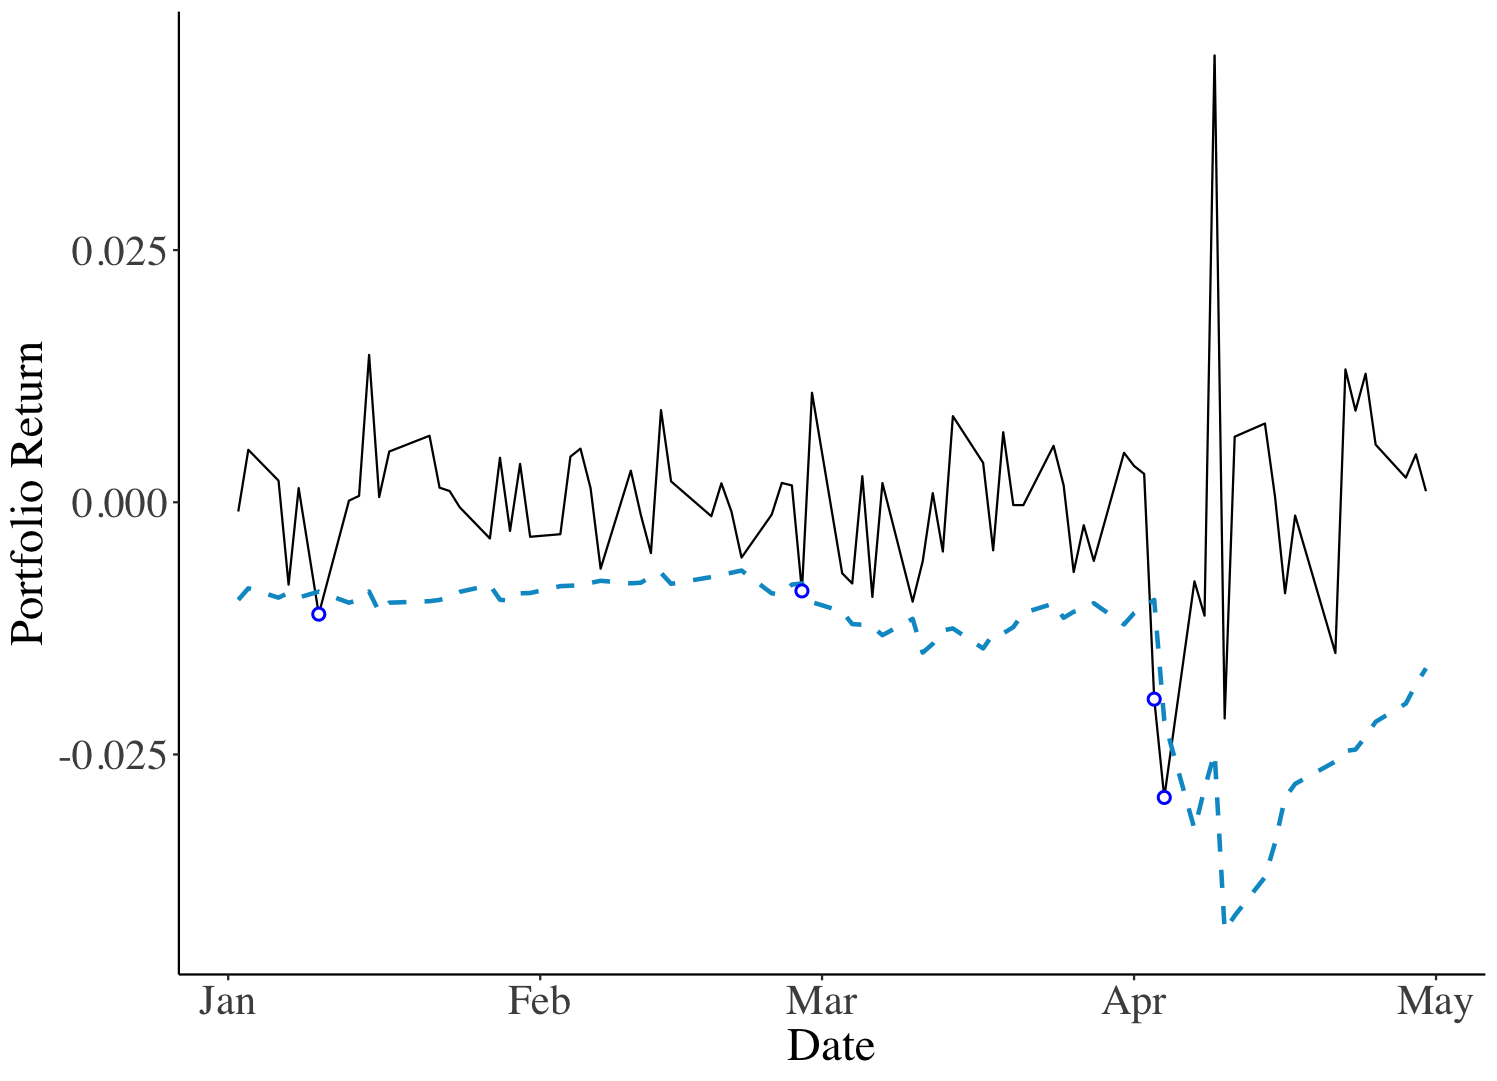
\includegraphics[width=0.95\linewidth]{5.6.png}
\column{0.49\textwidth}
\centering
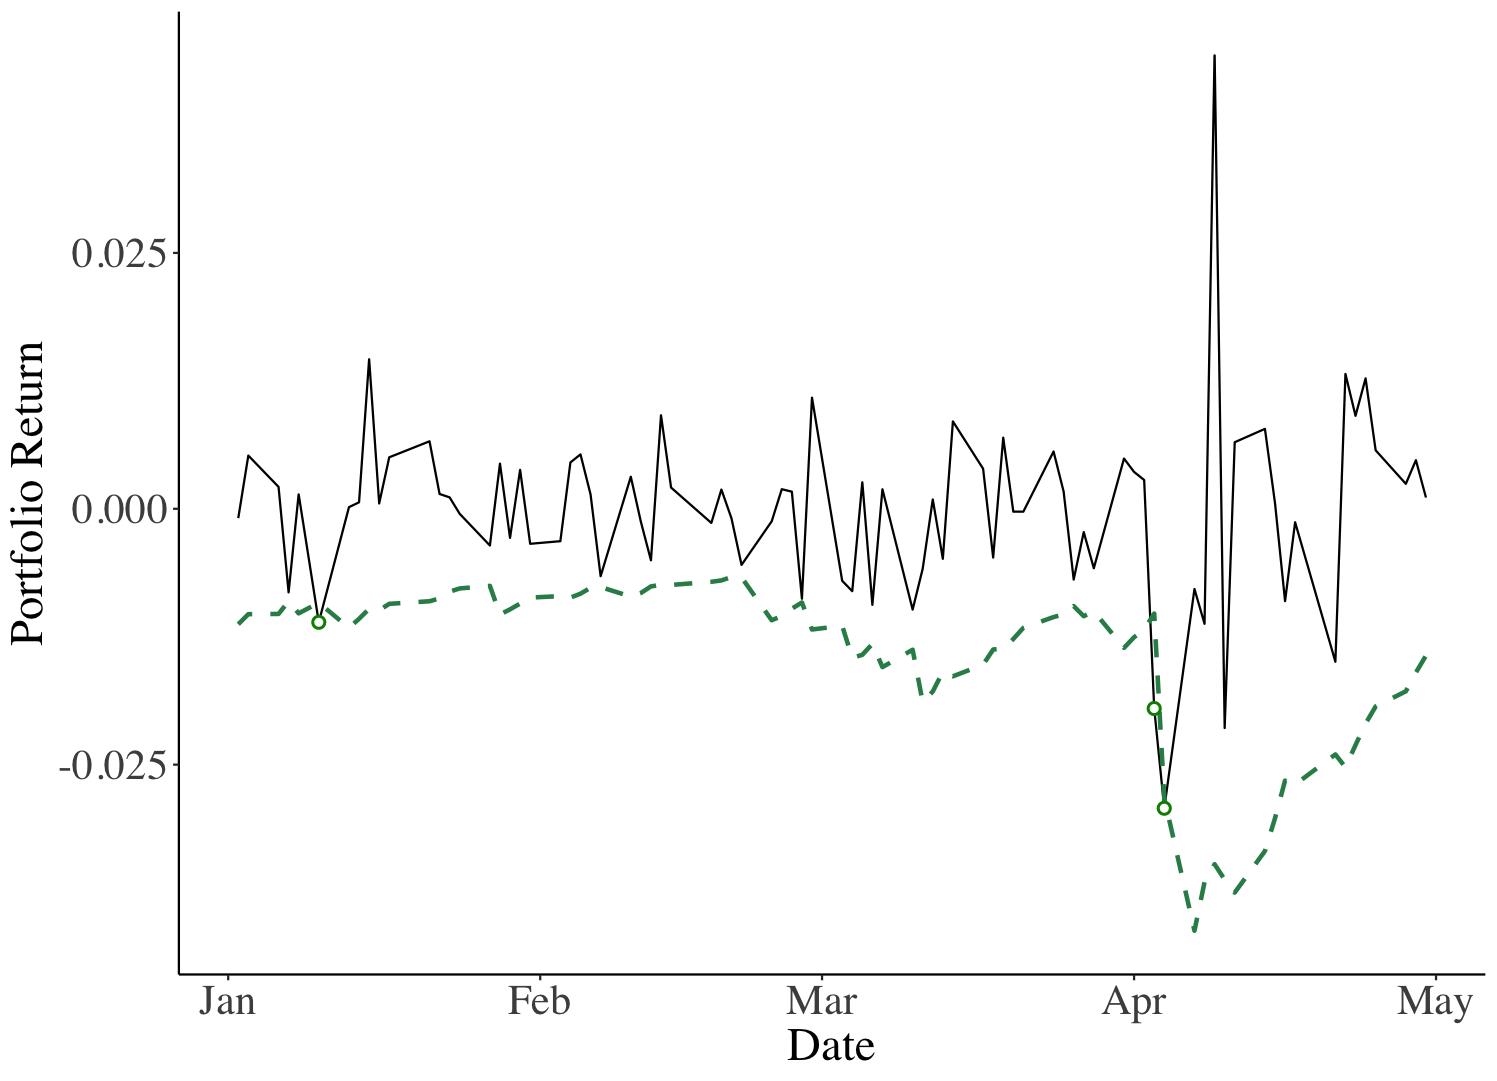
\includegraphics[width=0.95\linewidth]{5.7.png}
\end{columns}
\begin{itemize}
\item Breaches are similar across the two copula variants.
\item Main weakness remains clustering under abrupt volatility jumps.
\end{itemize}
\end{frame}

\begin{frame}{Copula Backtesting and Density Validation}
\begin{table}
\centering
\begin{tabular}{llcc}
\toprule
Test & p-value type & GARCH-GARCH & GJR-GJR \\
\midrule
\(LR_{\text{uc}}\) & Simulated & 0.188 & 0.554 \\
\(LR_{\text{ind}}\) & Simulated & 0.030 & 0.013 \\
\(LR_{\text{cc}}\) & Simulated & 0.217 & 0.200 \\
\bottomrule
\end{tabular}
\end{table}
\begin{itemize} \setlength{\itemsep}{1em}
\item KS on normal transform: \(p=0.5271\) (GARCH-GARCH), \(p=0.4872\) (GJR-GJR).
\item Density forecasts are statistically acceptable despite VaR clustering issues.
\end{itemize}
\end{frame}

\section{Conclusion}
\begin{frame}{Main Conclusions}
\begin{itemize}\setlength{\itemsep}{1em}
\item The thesis delivers a coherent end-to-end framework from univariate to multivariate risk modeling.
\item Volatility modeling: GJR improves in-sample volatility fit (QLIKE, LR evidence).
\item Shock modeling:
\begin{itemize}
\item Asymmetric t improves full-density fit.
\item EVT improves left-tail conservativeness for risk measures.
\end{itemize}
\item Backtesting reveals a persistent challenge: \textbf{independence of violations} under sudden volatility spikes.
\item Copula extension adds useful dependence structure and valid density forecasts for portfolios.
\end{itemize}
\end{frame}

\begin{frame}{Limitations and Next Steps}
\begin{itemize}\setlength{\itemsep}{1em}
\item Static dependence and symmetric copula limit adaptation and asymmetry capture.
\item EVT tails improve coverage but still react slowly to abrupt regime shifts.
\item Promising extensions:
\begin{itemize}
\item Dynamic/asymmetric copulas (\citeA{christoffersen2011joint}, \citeA{patton2011factor}).
\item Shock models with time-varying skewness and kurtosis.
\item Broader stress-testing and alternative volatility proxies.
\end{itemize}
\end{itemize}
\end{frame}

\begin{frame}[allowframebreaks]{References}
\bibliographystyle{apacite}
\nocite{Bollerslev2023,Campbell1997,Christoffersen2012,Tsay2010,Cont2001,Bollerslev1986,Glosten1993,Fernandez1998,mcneil2000estimation,christoffersen1998evaluating,diebold1998evaluating,berkowitz2001testing,diebold1995comparing,jondeau2006copulagarch,patton2006modelling,okimoto2008asymmetric,christoffersen2011joint}
\bibliography{\thesisbib}
\end{frame}

\begin{frame}[plain]
\centering
\Huge Questions
\vspace{1.2em}

\large \githubicon\ \href{https://github.com/ferpmillan/thesis}{github.com/ferpmillan/thesis}

\vspace{0.5em}

\large \githubicon\ \href{https://github.com/ferpmillan/thesis-tex}{github.com/ferpmillan/tesis-tex}
\end{frame}

\end{document}
